\documentclass{VUMIFPSkursinis}
\usepackage{algorithmicx}
\usepackage{algorithm}
\usepackage{algpseudocode}
\usepackage{amsfonts}
\usepackage{amsmath}
\usepackage{bm}
\usepackage{caption}
\usepackage{color}
\usepackage{float}
\usepackage{graphicx}
\usepackage{listings}
\usepackage{subfig}
\usepackage{wrapfig}
\usepackage{longtable}

\usepackage{datatool}% http://ctan.org/pkg/datatool
\newcommand{\sortitem}[2][\relax]{%
  \DTLnewrow{list}% Create a new entry
  \ifx#1\relax
    \DTLnewdbentry{list}{sortlabel}{#2}% Add entry sortlabel (no optional argument)
  \else
    \DTLnewdbentry{list}{sortlabel}{#1}% Add entry sortlabel (optional argument)
  \fi%
  \DTLnewdbentry{list}{description}{#2}% Add entry description
}
\newenvironment{sortedlist}{%
  \DTLifdbexists{list}{\DTLcleardb{list}}{\DTLnewdb{list}}% Create new/discard old list
}{%
  \DTLsort{sortlabel}{list}% Sort list
  \begin{itemize}%
    \DTLforeach*{list}{\theDesc=description}{%
      \item \theDesc}% Print each item
  \end{itemize}%
}

% Titulinio aprašas
\university{Vilniaus universitetas}
\faculty{Matematikos ir informatikos fakultetas}
\department{Programu sistemu katedra}
\papertype{Laboratorinis darbas}
\title{Festivaliu informacine sistema}
\titleineng{}
\status{2 kurso 5 grupes studentai}
\author{Mantas Petrikas}
\secondauthor{Olga Joana Šimitaite}   % Prideti antra autoriu
\thirdauthor{Migle Vaituleviciute}   % Prideti trecia autoriu
\fourthauthor{Vytautas Žilinas}   % Prideti ketvirta autoriu
\supervisor{Vytautas Valaitis}
\date{Vilnius – \the\year}

% Nustatymai
\setmainfont{Palemonas}   % Pakeisti teksto šrifta i Palemonas (turi buti idiegtas sistemoje)
\bibliography{bibliografija}

\begin{document}
\maketitle

\tableofcontents

\sectionnonum{Įvadas}

Lietuvoje vyksta daug festivalių, kurie savo informacija skelbia atskirose vietose, tačiau nėra patogios naudotis bendros informacines sistemos. 
Todėl atsižvelgę į tai nusprendėme, kad geriausia būtų sukurti tinklalapį, kuriame vartotojas galėtų lengvai bei efektyviai atrasti jį dominančią informaciją apie Lietuvoje vykstancius festivalius, taip padidinant žmonių susidomejimą Lietuvos festivaliais bei prisidedant prie jų garsinimo.

Šio, trečio laboratorinio darbo tikslas yra apibrežti tinklalio architektūra naudojant 4+1 architekturos pjūvių modelį, aprašant užduotis ir jų vykdymo scenarijus, strukturinį ir dinaminį tinkalapio modelius, tinklalapio komponentus ir komponentu išskirtyma tinkle, bei sukurti tinklalapio prototipą.  

\section{Užduotys ir jų vykdymo scenarijai}
Visame tinklalapyje yra keturi pagrindiniai agentai: vartotojas, festivalio organizatorius, administratorius ir žurnalistas. Šiame skyriuje išnagrinėsime visas šių agentų užduotis. Pirmiausia jas pavaizduosime atvejų diagrama, o vėliau visas užduotis parodysime sekų diagrama. 

Pirmasis agentas, kurį išnagrinėjome yra vartotojas, jis gali atlikti žemiau pateiktas užduotis.

\begin{figure}[H]
    \centering
    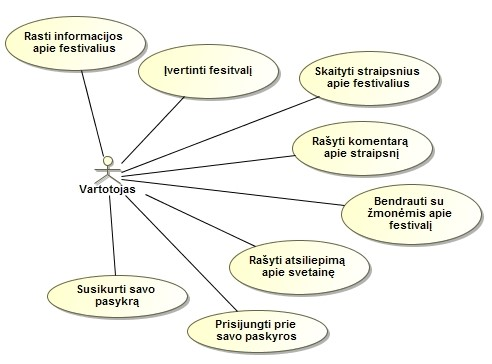
\includegraphics[scale=0.45]{img/Pav/Vartotojas}
    \label{img:uml1}
	\caption{Vartotojo užduotys}
\end{figure}

Vartotojas gali prisiregistruoti prie mūsų tinklalapio. Kad tai padarytų jam reikia atsidarius tinklalapį jo viršuje paspausti registracijos mygtuką, tada yra pateikiama registracijos formą, kurią jis privalo užpildyti. Ji yra išsiunčiama registracijos kontrolei, kuri išsaugo naują vartotoją duomenų bazėje. Ji atsako ar yra jau toks vartotojo vardas.  Jeigu toks vardas neegzistuoja, yra atidaroma vartotojo paskyrą, o jei toks vartotojo vardas egzistuoja tinklalapis vartotojui praneša, kad yra suvesti negalimi registracijos duomenys.

\begin{figure}[H]
    \centering
    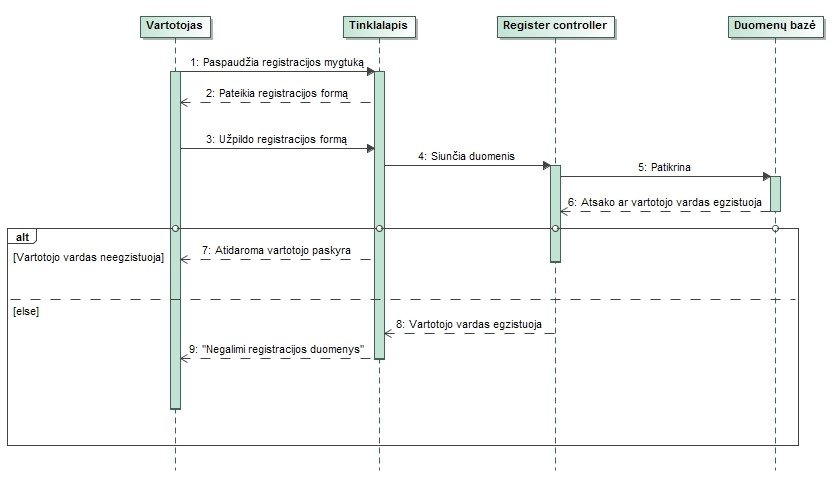
\includegraphics[scale=0.45]{img/Pav/VartotojoRegistracija}
    \label{img:uml2}
	\caption{Vartotojo registracijos seka}
\end{figure}

Vartotojas gali prisijungti prie tinklalapio. Kad tai padaryti vartotojas turi tinklalapio viršuje paspausti prisijungimo mygtuką. Tai padarius atsiveria prisijungimo langas, kurį užpildžius duomenys yra išsiunčiami į prisijungimo vadovą. Jis pateikia duomenis duomenų bazei patikrinti ar vartotojas egzistuoja. Jeigu toks vartotojas egzistuoja jam yra atidaroma jo paskyra, o jeigu tokio vartotojo nėra pranešama, kad vartotojas neegzistuoja su tokiais duomenimis.

\begin{figure}[H]
    \centering
    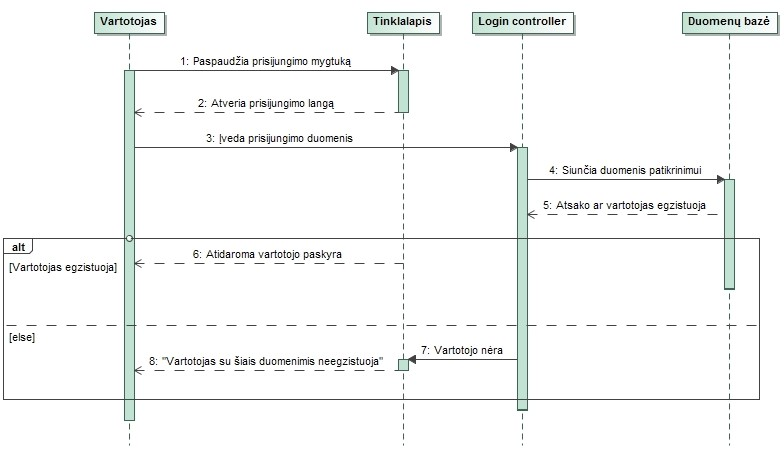
\includegraphics[scale=0.45]{img/Pav/VartotojoPrisijungimas}
    \label{img:uml3}
	\caption{Vartotojo prisijungimo seka}
\end{figure}

Vartotojas gali peržiūrėti festivalių sąrašą. Jis turi atsidaryti tinklalapį pasirinkti skiltį “Festivaliai”, tuomet tinklalapis prašo imti festivalių sąrašą iš vartotojo valdovo ( ang. User controller), kuris paima informaciją iš DB. Tada vartotojo valdovas siunčia informaciją tinklalapiui, kuris ją atvaizduoja vartotojui.
Jeigu vartotojas nori daugiau informacijos apie festivalį, jis turi pasirinkti festivalį. Tada jo ID yra siunčiama vartotojo valdovui, kuris iš DB paima to festivalio informaciją ir tada ją siunčia tinklalapiui. Šis atidaro naują langą su visa informacija. Taip pat, vartotojas gali rašyti komentarus  prie festivalių arba juos vertinti. Tačiau tai gali daryti tik prisijungę vartotojai. Jeigu vartotojas yra prisijungęs jam yra leidžiama naudotis festivalio komentarų bei vertinimo erdve, tada jis gali parašyti komentarą arba vertinimą, kuriuos siunčia į vartotojo vadovą, kuris komentarą arba vertinimą saugo į DB. Vartotojo vadovas patvirtina, kad duomenys yra įkelti. Ir tada tinklalapyje atsiranda komentaras arba vertinimas. Tačiau jeigu vartotojas neturi paskyros jam tinklalapis rašo, kad norint komentuoti arba vertinti reikia turėti paskyrą.

\begin{figure}[H]
    \centering
    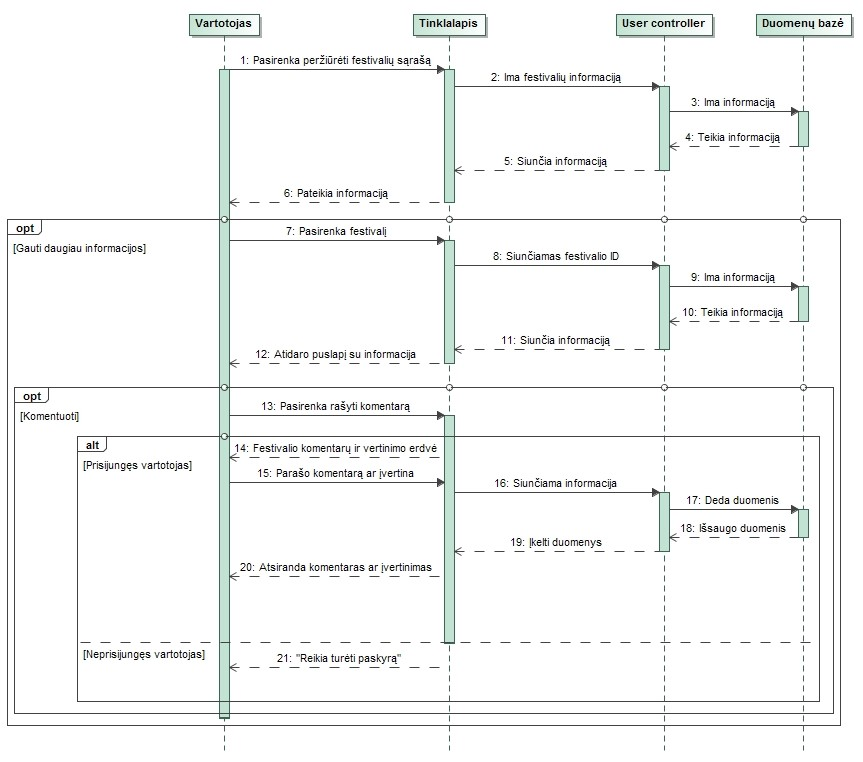
\includegraphics[scale=0.45]{img/Pav/VartotojoInfoFest_Komentarai}
    \label{img:uml4}
	\caption{Vartotojo veiksmai su festivaliais}
\end{figure}

Vartotojas gali peržiūrėti visus straipsnius. Tai gali padaryti atsidarydamas tinklalapį ir pasirinkdamas skiltį “Naujienos”. Tada tinklalapis siunčia prašymą vartotojo vadovui, kuris iš duomenų bazės ima informaciją ir ją siunčia į tinklalapį, kuris ją pateikia vartotojui. Jeigu vartotojas nori perskaityti visą straipsnį, spaudžia “Skaityti daugiau” ir tada tinklalapis siunčia straipsnio ID vartotojo vadovui, kuris ima informaciją apie tą straipsnį ir jį siunčia į tinklalapį, kuris naujame puslapyje vartotojui parodo straipsnį.
	Beje, jei vartotojas yra prisijungęs jis gali rašyti komentarą. Šis komentaras yra siunčiamas vartotojo vadovui, kuris įkelia komentarą į DB. Tada, vartotojo vadovas tinklalapiui praneša apie sėkmingą išsaugojimą ir tinklalapyje atsiranda komentaras. Tačiau jei vartotojas nėra prisijungęs tinklalapis jam praneša, kad reikia būti prisijungusiam.

\begin{figure}[H]
    \centering
    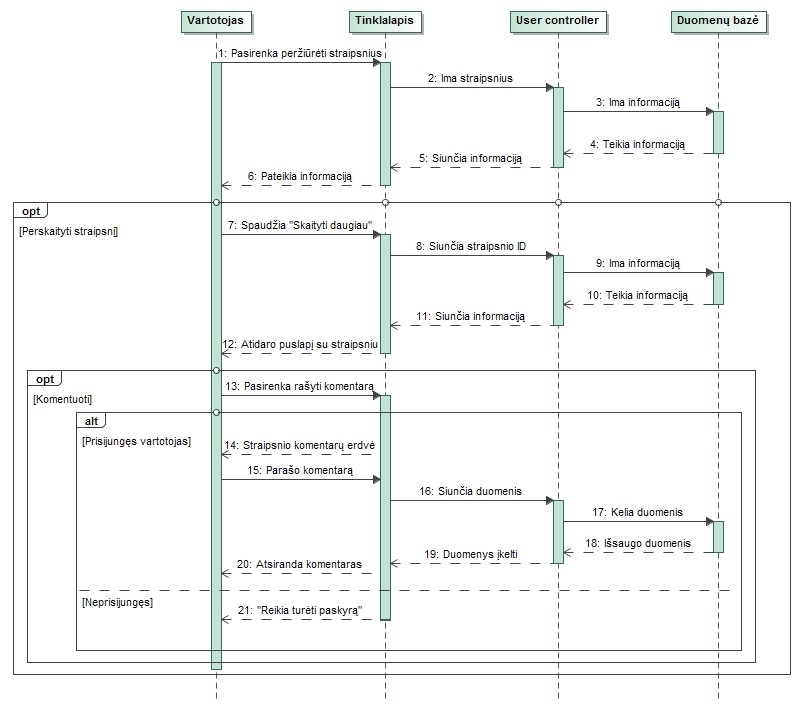
\includegraphics[scale=0.45]{img/Pav/VartotojasStraips_Komentarai}
    \label{img:uml5}
	\caption{Vartotojo veiksmai su straipsniais}
\end{figure}	
	
Vartotojas gali parašyti atsiliepimą. Tai padaryti jis gali atsidaręs tinklalapį ir pasirinkęs skiltį “Apie mus”. Ten jis parašo atsiliepimą, kuris su vartotojo ID yra siunčiami vartotojo vadovui, kuris saugo informaciją į DB. Ir kai saugojimas yra įvykdytas vartotojo vadovas praneša apie sėkmingą įkėlimą tinklalapiui, kuris informuoja vartotoją. Kadangi yra reikalingas ir vartotojo ID, atsiliepimus gali rašyti tik prisijungę vartotojai.
	
\begin{figure}[H]
    \centering
    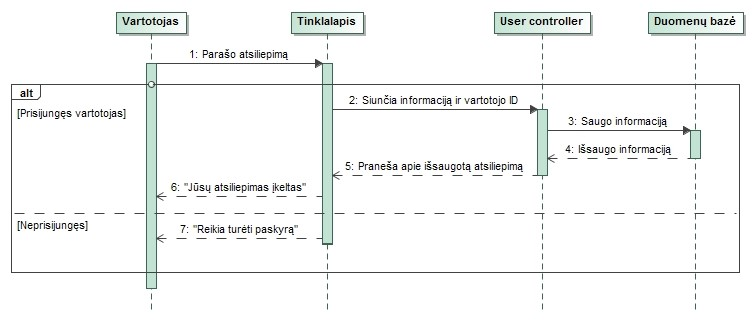
\includegraphics[scale=0.45]{img/Pav/VartotojasAtsiliepimas}
    \label{img:uml6}
	\caption{Vartotojo atsiliepimų seka}
\end{figure}	
	
Sekantis agentas yra festivalio organizatorius su vienu tikslu.

\begin{figure}[H]
    \centering
    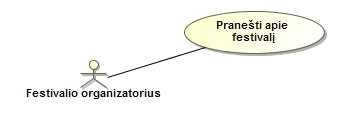
\includegraphics[scale=0.45]{img/Pav/FestivalioOrg}
    \label{img:uml7}
	\caption{Festivalio organizatoriaus užduotis}
\end{figure}	
	
Festivalio organizatorius gali atlikti tik vieną užduotį. Tai yra pranešti apie festivalį. Jis tai gali padaryti atsidaręs tinklalapį ir pasirinkęs skiltį “Festivaliai” ir ten paspaudęs ant mygtuko “Pranešti apie festivalį”. Tuomet tinklalapis pateikia festivalio formą, kurią festivalio organizatorius užpildo ir visa informacija yra išsiunčiama į Admin panel.

\begin{figure}[H]
    \centering
    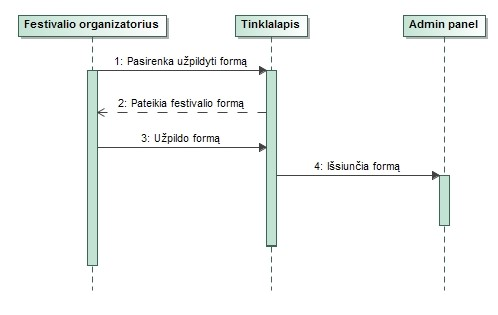
\includegraphics[scale=0.45]{img/Pav/FestivalOrgPranesti}
    \label{img:uml8}
	\caption{Festivalio organizatoriaus veiksmų seka}
\end{figure}	

Dar vienas agentas yra administratorius su daugiausia užduočių mūsų tinklalapyje. Jis paveldi visas žurnalisto užduotis.

\begin{figure}[H]
    \centering
    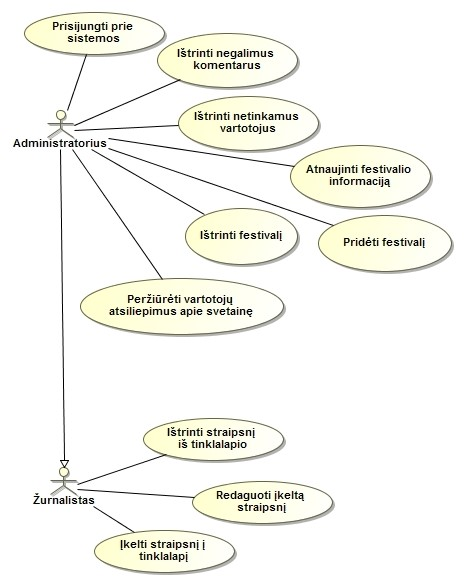
\includegraphics[scale=0.45]{img/Pav/Administratorius}
    \label{img:uml9}
	\caption{Administratoriaus užduotys}
\end{figure}	

Administratorius gali prisijungti prie sistemos. Tai padaryti jis gali, kai užpildo prisijungimo formą, kurią pateikia admin panel. Ji prisijungimo duomenis siunčia DB vadovui (ang. DB controller), kuris juos tikrina DB’ėje. Jeigu duomeys yra tinkami yra leidžiama naudotis admin panel, o jeigu duomenys nėra rasti - pranešama, kad tokių duomenų nėra sistemoje.

\begin{figure}[H]
    \centering
    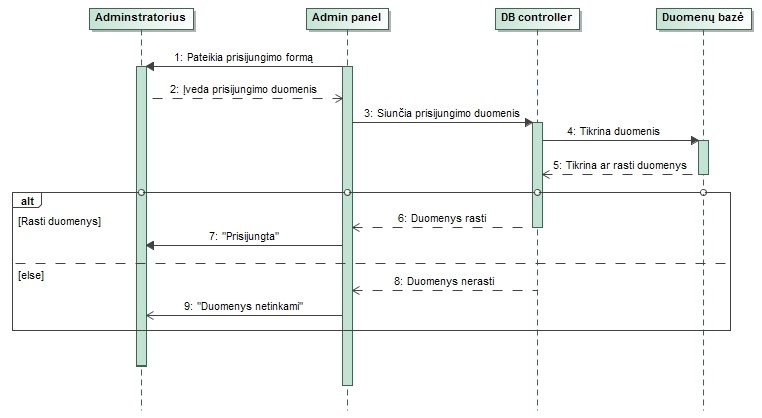
\includegraphics[scale=0.45]{img/Pav/AdminPrisijungtiPrieSis}
    \label{img:uml10}
	\caption{Administratoriaus prisijungimo veiksmų seka}
\end{figure}

Administratorius gali pridėti festivalį, kurį atsiuntė į sistemą festivalio organizatorius. Jis tai gali padaryti paspaudęs mygtuką “Pridėti festivalį”, tuomet admin panel pateikia festivalio formą, kurią administratorius užpildo pagal atsiųsta informaciją. Tuomet ta informacija yra siunčiama DB vadovui, kuris ją išsaugo DB ir įkelia tą festivalį į tinklalapį bei praneša admin panel apie sėkmingą įkėlimą, o ši informuoja administratorių.

\begin{figure}[H]
    \centering
    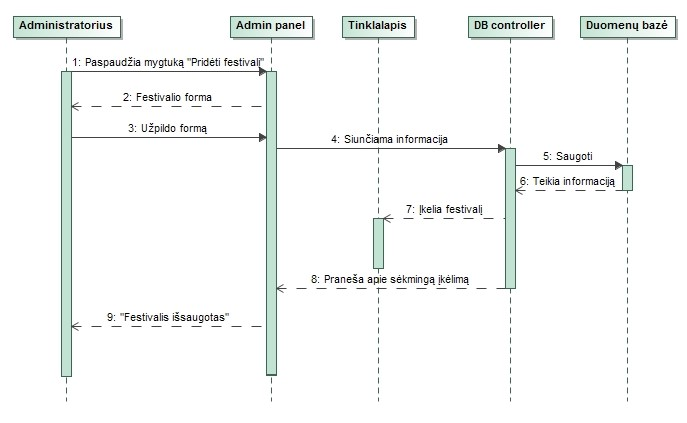
\includegraphics[scale=0.45]{img/Pav/AdminPridetiFestivali}
    \label{img:uml11}
	\caption{Administratorius prideda festivalį}
\end{figure}
	
Administratorius gali peržiūrėti visus publikuotų festivalių skelbimus. Tai gali padaryti pasirinkęs peržiūrėti festivių sąrašą. Tada, admin panel prašo gauti informacijos DB vadovui, o jis iš DB ima ir siunčia informaciją admin panel, kad ji informaciją pateiktų administratoriui. Tada administratorius gali pasirinkti festivalį ir padaryti tokius pasirinkimus: 
\begin{itemize}
\item Ištrinti festivalį. Tada admin panel nusiunčia festivalio ID DB vadovui, kuris ištrina festivalį iš DB ir praneša apie sėkmingą funkcijos atlikimą. Ir admin panel praneša administratoriui apie festivalio ištrinimą;
\item Atnaujinti festivalį. Tada yra nusiunčiamas festivalio ID ir DB vadovas gauna informaciją iš DB ir ją siunčia į admin panel, kuri pateikią festivalio informacijos forma administratoriui. Tuomet administratorius gali pakeisti to festivalio infromaciją ir ją išsaugoti. Tada admin panel siunčia informaciją DB vadovui, kuris atnaujina informaciją DB ir praneša apie sėkmingą atnaujinimą, o admin panel praneša apie tai administratoriui. 
\end{itemize}
	
\begin{figure}[H]
    \centering
    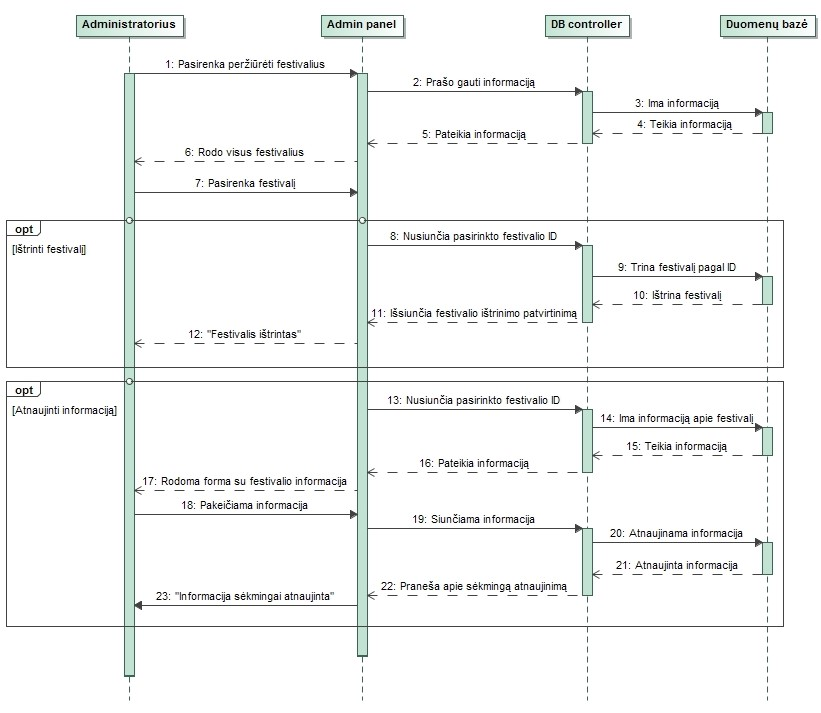
\includegraphics[scale=0.45]{img/Pav/AdminIstrintiAtnaujintiFest}
    \label{img:uml12}
	\caption{Administratorius veiksmai su festivaliais}
\end{figure}	
	
Administratorius gali ištrinti vartotojus, kurie pastoviai nusižengia tinklalapio taisyklėms. Tai jis gali padaryti pasirinkdamas, kad jam parodytų vartotojų sąrašą. Admin panel prašo dauti informacijos DB vadovo, o šis ima informaciją iš DB ir ją siunčia atgal į admin panel. O admin panel pateikia sąrašą administratoriui. Jis gali pasirinkti vartotoją. Tada to vartotojo ID yra siunčiamas DB vadovui, kuris paima to vartotojo informaciją iš DB ir ją siunčia į admin panel. Tada admin panel atidaro naują langą su visa statistine informaciją apie vartotoją. Jeigu administratorius nusprendžia, kad vartotoją reikia ištrinti jis pasirenka tokia funkciją ir admin panel išsiunčia to vartotojo ID DB vadovui, kuris pašalina iš DB tą vartotoją ir visą informaciją su juo bei gražina, kad funkcija sėkmingai įvykdyta.

\begin{figure}[H]
    \centering
    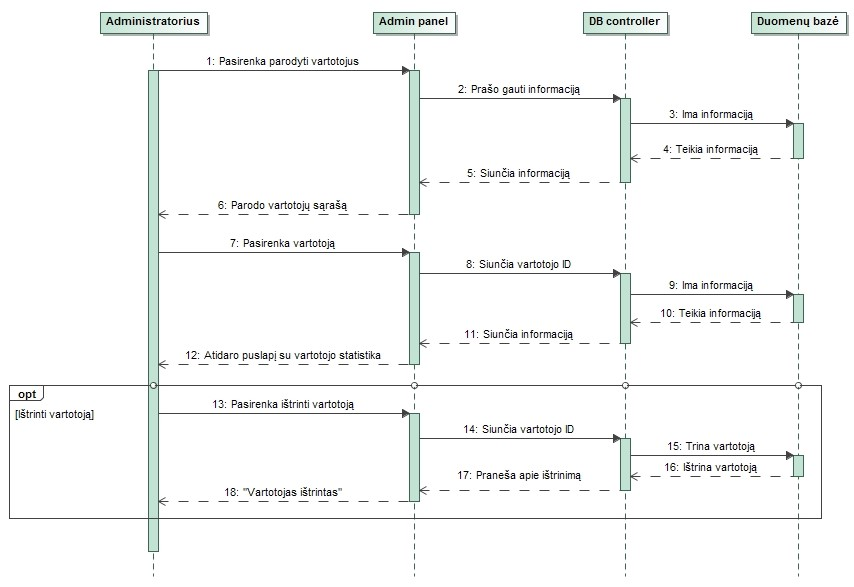
\includegraphics[scale=0.45]{img/Pav/AdminIstrintiVartotoja}
    \label{img:uml13}
	\caption{Administratorius ištrina vartotoją}
\end{figure}	
	
Administratorius gali ištrinti netinkamą komentarą. Tai padaryti jis gali, kai pasirenka, kad jam admin panel rodytų visus komentarus bei gali pasirinkti pagal ką jam bus rodomi komentarai: nauji nuo paskutinio patikrinimo, nuo tam tikros datos ar tam tikro festivalio (straipsnio) ir t.t.. Tada admin panel prašo gauti informaciją DB vadovo, jis paima informaciją iš DB ir siunčia į admin panel, kuri sąrašą atvaizduoją administratoriui. Kai administratorius pasirenka komentarą, admin panel siunčia to komentaro ID DB vadovui ir šis iš DB ištrina tą komentarą bei praneša apie sėkmingą ištrinimą. Admin panel parodo pranešimą, kad komentaras ištrintas, administratoriui. 
	Tačiau administratorius gali peržvelgti tik tuos komentarus, kuriuos pranešė kiti vartotojai. Jis pasirenka šia opciją ir admin panel prašo DB vadovo, kad duotų informacijos ir šis paima ją iš DB ir siunčia admin panel, kuri administratoriui juos parodo. Tada administratorius pasirenka netinkamus ir ištrina. Admin panel siunčia komentarų ID ir DB vadovas juos ištrina iš DB ir praneša apie sėkimingą funkcijos įvykdymą.

\begin{figure}[H]
    \centering
    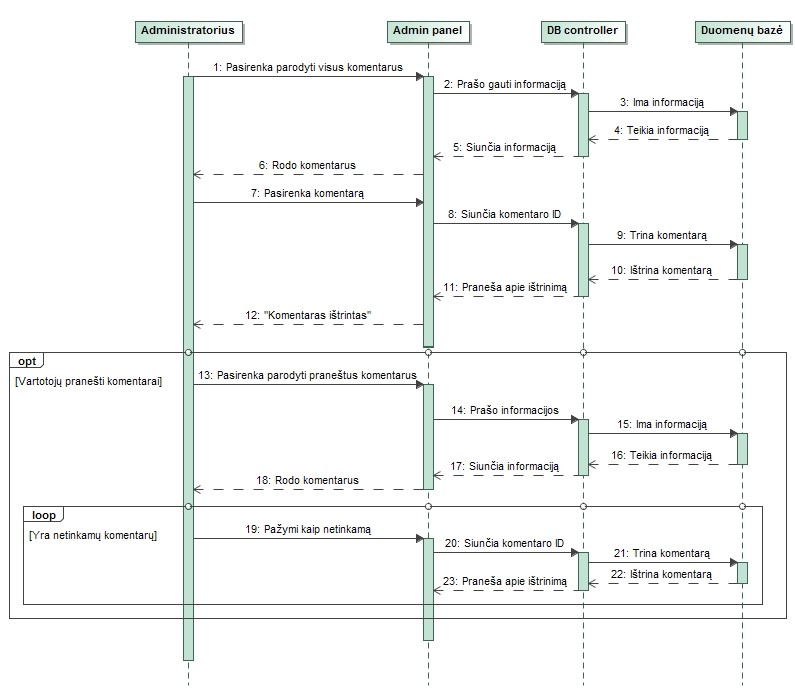
\includegraphics[scale=0.45]{img/Pav/AdminIstrintiKomentarus}
    \label{img:uml14}
	\caption{Administratorius ištrina komentarą}
\end{figure}	
	
Administratorius gali peržiūrėti visus vartotojų atsiliepimus. Jis turi pasirinkti tokią opciją ir tada admin panel prašo DB vadovo suteikti tokią informaciją. Tada DB vadovas paima informaciją iš DB ir ją išsiunčia į admin panel, kuri šią informaciją atvaizduoja. Tada, administratorius gali ištrinti bereikšmius atsiliepimus iš sistemos. Jis turi pasirinkti atsiliepimą, tada to atsiliepimo ID yra išsiunčiamas DB vadovui, kuris ištrina atsiliepimą iš DB ir praneša apie sėkmingą to atlikimą. Ir tada admin panel apie tai praneša administratoriui.
	
\begin{figure}[H]
    \centering
    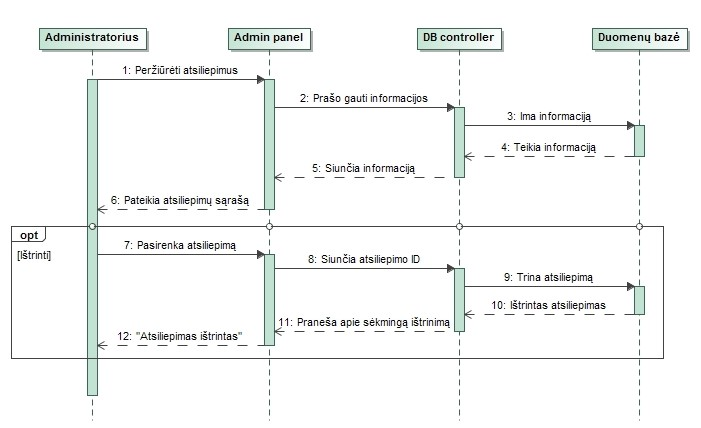
\includegraphics[scale=0.45]{img/Pav/AdminAtsiliepimaiSvetaine}
    \label{img:uml15}
	\caption{Administratorius peržiūri atsiliepimus}
\end{figure}
	
Paskutinis agentas mūsų tinklalapyje yra žurnalistas, kurio užduotis turi ir administratorius.

Žurnalistas gali įkelti straipsnį į tinklalapį. Tai padaro pasirinkdamas įkelti straipsnį, tada zurnalistas panel pateikia straipsnio formą, kurią žurnalistas užpildęs deda į sistemą. Zurnalistas panel siunčia informaciją DB vadovui, kuris saugo informaciją į DB ir taip pat ima informaciją iš DB tam, kad galėtų automatiškai įkelti į tinklalapį. O apie sėkmingą įkėlimą zurnalistas panel praneša žurnalistui.

\begin{figure}[H]
    \centering
    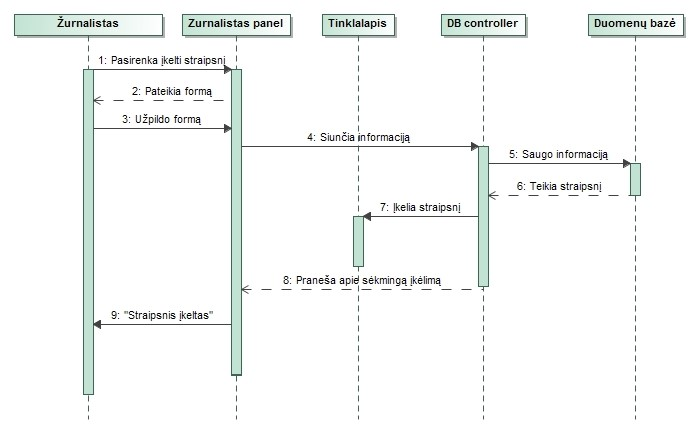
\includegraphics[scale=0.45]{img/Pav/ZurnalistasIkeliaStraipsni}
    \label{img:uml16}
	\caption{Žurnalistas įkelia straipsnį}
\end{figure}

Žurnalistas gali ir peržvelgti visus straipsnius. Kai žurnalistas pasirenka tokią galimybę zurnalistas panel prašo informacijos DB vadovo, kuris ją ima iš DB ir siunčia atgal į zurnalistas panel, o ši pateikia sąrašą žurnalistui. Tada žurnalistas pasirenka straipsnį ir jis gali pasirinkti ką, daryti:
\begin{itemize}
\item Ištrinti. Tada zurnalistas panel siunčia straipsnio ID DB vadovui, kuris ištrina straipsnį iš DB ir praneša apie sėkmingą ištrinimą. O zurnalistas panel praneša apie straipsio ištrinimą žurnalistui.
\item Redaguoti. Zurnalistas panel siunčia straipsnio ID DB vadovui, kuris ima informaciją iš DB ir ją siunčia į zurnalistas panel, kuri straipsnio formą pateikia žurnalistui. Jis gali redaguoti visą straipsnio informaciją, o baigęs išsaugoti. Tada zurnalistas panel siunčia informaciją DB vadovui, kuris atnaujina straipsnio informaciją ir apie sėkmingą atnaujinimą praneša. O zurnalistas panel praneša apie sėkmingą atnaujinimą žurnalistui.
\end{itemize}	
	
\begin{figure}[H]
    \centering
    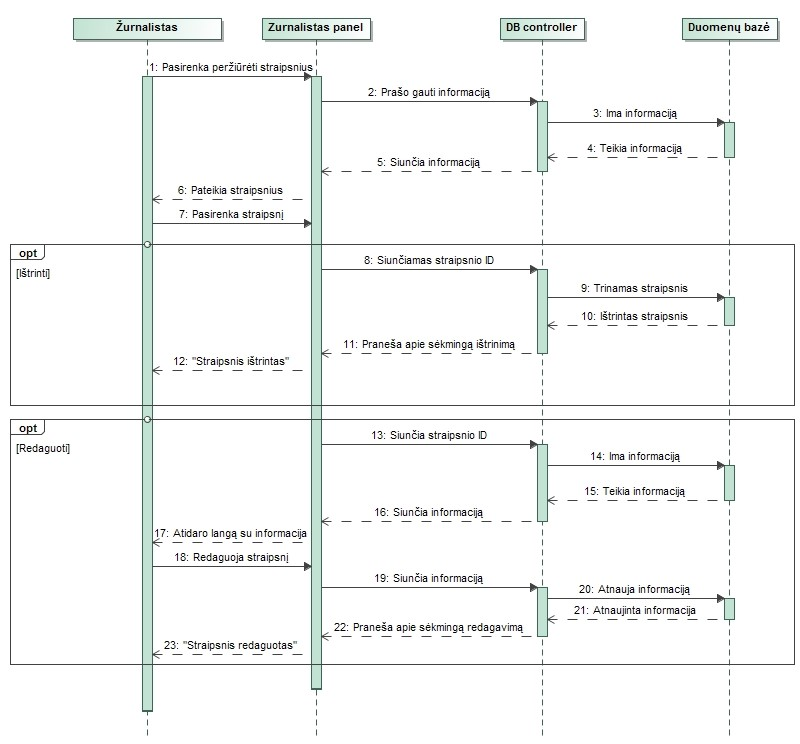
\includegraphics[scale=0.45]{img/Pav/ZurnalistasIstrina_Redaguoja}
    \label{img:uml16}
	\caption{Žurnalisto atliekamų veiksmų sekos}
\end{figure}	
	
\section{Struktūrinis programų sistemos modelis}
Šiame skyriuje nagrinėjamas funkcinių reikalavimų įgyvendinimas, vaizduojamos informacinę festivalių sistemą sudarančios klasės ir jų sąryšiai.

Pirmiausiai pateikiama UML paketų diagrama, kurioje vaizduojamos viso klasės ir jų skirstymas į paketus.
\begin{center}
    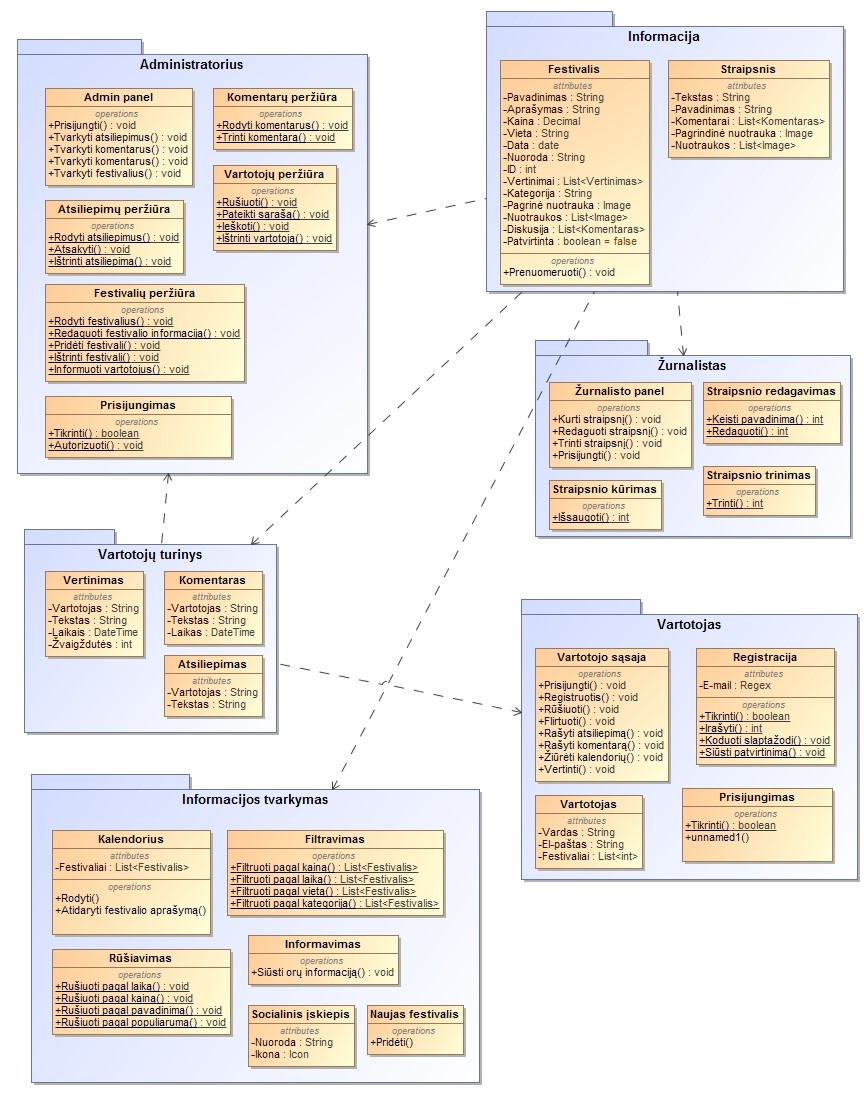
\includegraphics[scale=0.5]{img/PSI3/paketai}
	\label{img:uml17}
	\caption{???????????}
\end{center}

Toliau pateiktoje klasių diagramoje vaizduojami klasių, apibrėžiančių administratoriui skirtas funkcijas, ryšiai. \textit{Admin panel} klasė paveldi iš \textit{Žurnalisto panel} klasės, nes ir administratorius gali atlikti visas žurnalisto užduotis.
\begin{center}
    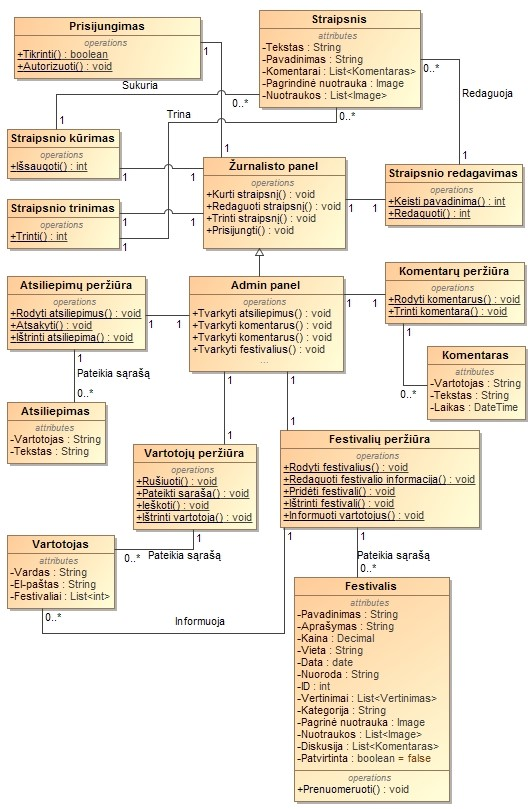
\includegraphics[scale=0.5]{img/PSI3/admin}
	\label{img:uml18}
	\caption{???????????}
\end{center}
Pagrindinė klasė, leidžianti atlikti žurnalisto užduotis, yra \textit{Žurnalisto panel}. \textit{Žurnalisto panel} naudoja klases: \textit{Straipsnio kūrimas, Straipsnio redagavimas, Straipsnio trynimas}. Šios klasės turi prieigą prie duomenų bazėje saugomų straipsnių, todėl yra susijusios su klase \textit{Straipsnis}. \textit{Žurnalisto panel} taip pat naudoja klasę \textit{Prisijungimas}.
Pagrindinė klasė, leidžianti atlikti administratoriaus užduotis, yra \textit{Admin panel}. Be klasių, kurias naudoja \textit{Žurnalisto panel} klasė, \textit{Admin panel} naudoja klases: \textit{Atsiliepimų peržiūra, Vartotojų peržiūra, Komentarų peržiūra, Festivalių peržiūra}. Kadangi šiose klasėse yra metodai leidžiantys dirbti su duomenų bazėje saugoma informacija, klasė \textit{Atsiliepimų peržiūra} yra susijusi su klase \textit{Atsiliepimas}, \textit{Vartotojų peržiūra} - su \textit{Vartotojas}, \textit{Komentarų peržiūra} - su \textit{Komentaras} bei \textit{Festivalių peržiūra} - su \textit{Festivalis}. \textit{Festivalių peržiūra} yra susijusi su klase \textit{Vartotojas}, nes klasėje \textit{Festivalių peržiūra} yra metodas, leidžiantis siūsti informaciją visiem tam tikrą festivalį užsiprenumeravusiems vartotojams.

Žemiau pateiktoje diagramoje vaizduojamas klasių, leidžiančių informuoti vartotoją apie oro sąlygas likus trim dienom iki festivalio, sąryšis.
\begin{center}
    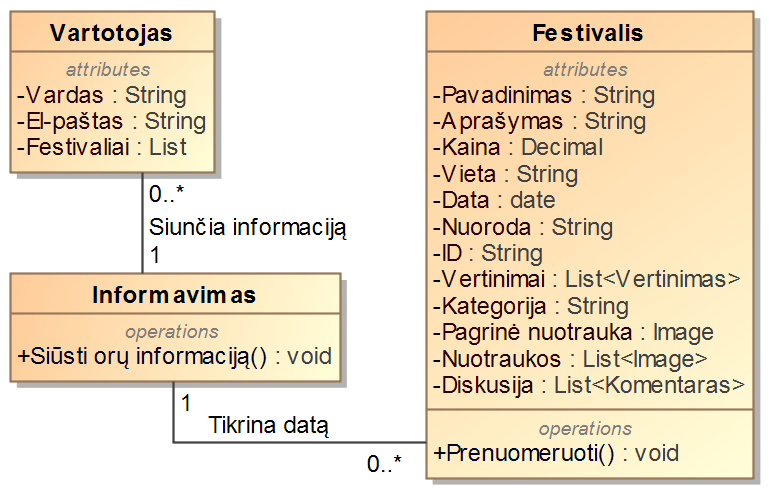
\includegraphics[scale=0.5]{img/PSI3/orai.PNG}
	\label{uml:19}
	\caption{?????????}
\end{center}
Klasė \textit{Informavimas} yra susijusi su klase \textit{Festivalis}, nes tikrina festivalių datas. Kadangi klasė \textit{Informavimas} turi metodą, leidžiantį siųsti informaciją vartotojams, yra susijusi su klase \textit{Vartotojas}.

Toliau pateikiama naujo festivalio įtraukimo į duomenų bazę diagrama.
\begin{center}
    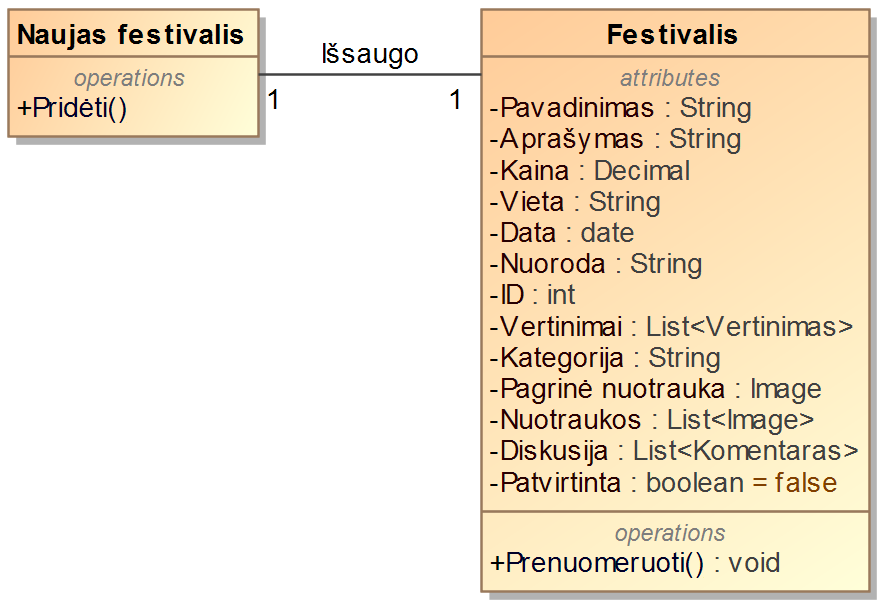
\includegraphics[scale=0.5]{img/PSI3/naujas.PNG}
	\label{uml:20}
	\caption{?????????}
\end{center}
Kai užpildoma anketa apie naują festivalį, naujas \textit{Festivalis} yra įtraukiamas į duomenų bazę. Kol administrsatorius nepatikrina pateiktos informacijos \textit{Patvirtinta} turi vertę \textit{false}.

Toliau pateiktoje klasių diagramoje vaizduojami klasių, apibrėžiančių vartotojui skirtas funkcijas, ryšiai.
\begin{center}
    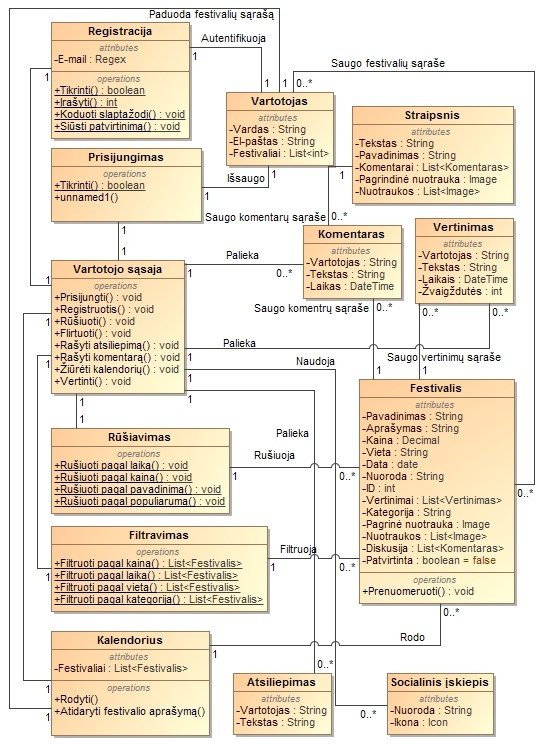
\includegraphics[scale=0.5]{img/PSI3/user}
	\label{uml:21}
	\caption{?????????}
\end{center}
Pagrindinė klasė, leidžianti atlikti vartotojo užduotis, yra \textit{Vartotojo sąsaja}. \textit{Vartotojo sąsaja} yra susijusi su klasėmis: \textit{Prisijungimas, Registracija, Kalendorius, Rūšiavimas, Filtravimas, Socialinis įskiepis, Komentaras, Vertinimas, Atsiliepimas}. Klasė \textit{Prisijungimas} gali tikrinti vartotojų sąrašą, o \textit{Registracija} - pridėti naujus vartotojus, todėl šios klasės yra susijusios su klase \textit{Vartotojas}. Klasė \textit{Komentaras} yra susijusi su klase \textit{Straipsnis}, nes \textit{Straipsnis} saugo komentarų sąrašą. Klasės \textit{Komentaras} ir \textit{Vertinimas} yra susijusios su klase \textit{Festivalis}, nes \textit{Festivalis} saugo komentarų ir vertinimų sąrašus. Klasė \textit{Kalendorius} yra susijusi su klase \textit{Festivalis}, nes \textit{Kalendorius} saugo vartotojo pasirinktus festivalius. \textit{Kalendorius} turi sąryšį su klase \textit{Vartotojas}, nes atvaizdavimui naudoja vartotojo festivalių sąrašą. Klasės \textit{Rūšiavimas} ir \textit{Filtravimas} yra susijusios su klase \textit{Festivalis}, nes jos pertvarko vartotojui rodomą festivalių sąrašą.

\section{Dinaminis programų sistemos modelis}

Šiame skyrelyje apžvelgsime, kaip tinklalapio veikimo metu veikia aplikacija ir keičiasi kelių jos elementų būsenos. Tai atlikome naudodami veiklos diagramas, pritaikydami jas pagrindiniams tinklalapio procesams, ir būsenos diagramas, pritaikę jas tinklalapiui ir vartotojui.


Žemiau pateikta veiklos diagrama, kuri rodo ką vartotojas gali daryti tinklalapyje pasirinkęs “Festivaliai” skiltį. Vartotojas gali tiesiog ieškoti straipsnio eidamas per visą skiltį arba jis gali tikslingai pasirinkti rikiavimo arba filtravimo būdą, arba žinodamas festivalio pavadinimą - jį gali įvesti į paieškos laukelį. Iš atrinktų festivalių vartotojas gali toliau rinktis festivalį. O tada gali išsirinkti vieną festivalį ir arba jis randa informaciją, kurios ir ieškojo, arba, jeigu vartotojas yra prisijungęs, jis gali įvertinti festivalį, diskutuoti su žmonėmis arba užsiprenumeruoti festivalį. Jeigu vartotojas užsiprenumeruoja festivalį, tada likus trims dienoms iki festivalio jam yra pranešama, kokia bus meteorologinė situacija festivalio metu.

\begin{figure}
	\centering
    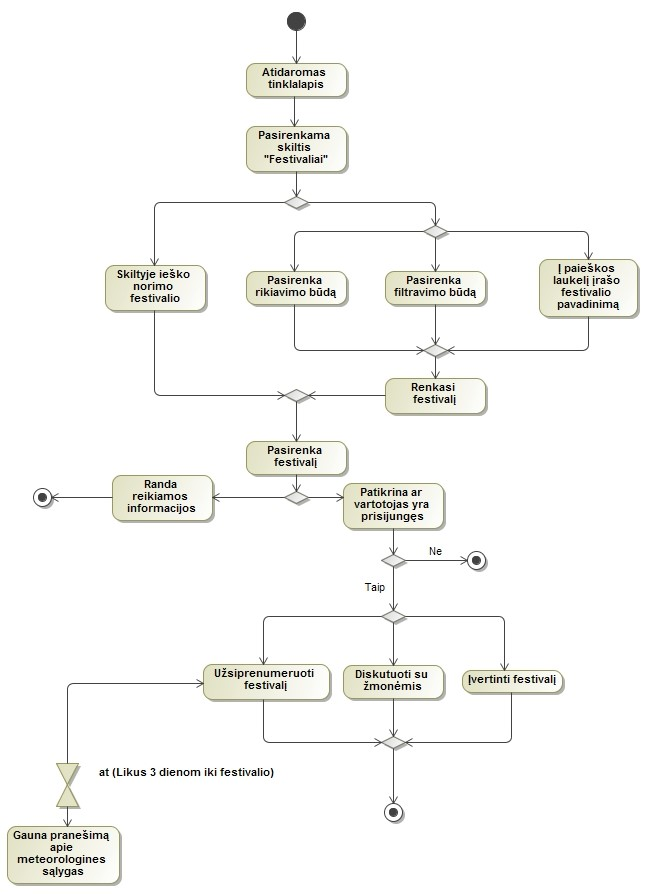
\includegraphics[scale=0.5]{img/Pav/VartotojasFestivalis}
	\label{uml:22}
	\caption{Vartotojo veiksmai "Festivaliai" skiltyje}
\end{figure}

Beje, vartotojas gali pasirinkti skiltį “Naujienos”. Tada jis gali ieškoti straipsnio, jeigu jis randa straipsnį, kurį nori perskaityti - spaudžia “Skaityti daugiau”. Tada gali perskaityti straipsnį ir jeigu nori bei yra prisijungęs vartotojas gali komentuoti. Arba gali eiti toliau ieškoti straipsnio.

\begin{figure}
	\centering
    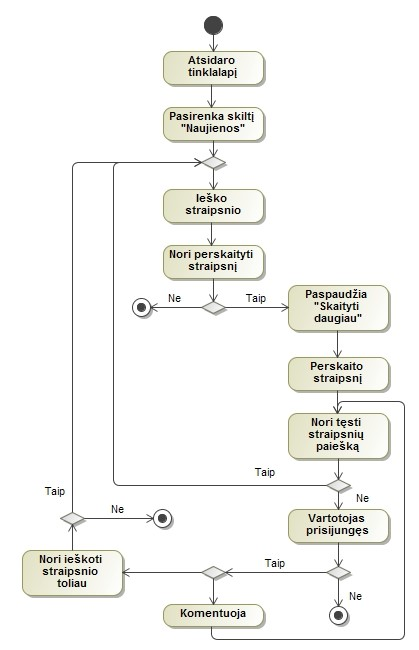
\includegraphics[scale=0.5]{img/Pav/VartotojasStraipsnis}
	\label{uml:23}
	\caption{Vartotojo veiksmai "Naujienos" skiltyje}
\end{figure}

Vartotojas atsidaręs tinklalapį, jei turi paskyrą gali prie jos prisijungti. Tai padaro paspausdamas prisijungimo mygtuką ir įvesdamas prisijungimo duomenis ir taip prisijungia. Tačiau jei jis neturi savo paskyros vartotojas gali paspausti registracijos mygtuką ir tada gali pasirinkti naudoti įskiepius, jeigu nenori jis užpildo registracijos formą, o jeigu nori naudoja įskiepius. Ir taip susikuria paskyrą.
	Prisijungęs ar susikūręs pasykrą vartotojas gali paspausti ant “Mano meniu” mygtuko ir tada gali rinktis ką nori daryti:
\begin{itemize}
\item Gali paspausti ant mygtuko “Mano kalendorius” ir tada pamato jo pasirinktus festivalius kalendoriuje. Jeigu jis nori gauti informacijos vartotojas paspaudžia ant festivalio ir atsiranda langas su festivalio informacija.
\item Gali paspausti ant “Nauji pranešimai” mygtuko ir tada jeigu yra naujų pranešimų jie yra matomi, o jeigu jų nėra, tada būna parašyta, kad naujų pranešimų nėra. 
\item Gali pasirinkti “Užsiprenumeruoti festivaliai” pasirinkties ir tada vartotojas mato sąrašą festivalių, kuriuos jis užsiprenumeravęs. Jeigu nori gali paspausti ant festivalio ir sužinoti daugiau informacijos apie jį.
\item Gali paspausti ant “Nustatymai”. Tada vartotojas gali pakeisti savo paskyros duomenis (slapyvardis, slaptažodis, paskyros paveikslėlį) arba gali pakeisti “Domina” nustatymus.
\end{itemize}
 Visais atvejais vartotojas gali grįžti į “Mano meniu” ir tęsti veiklą.
 
\begin{figure}
	\centering
    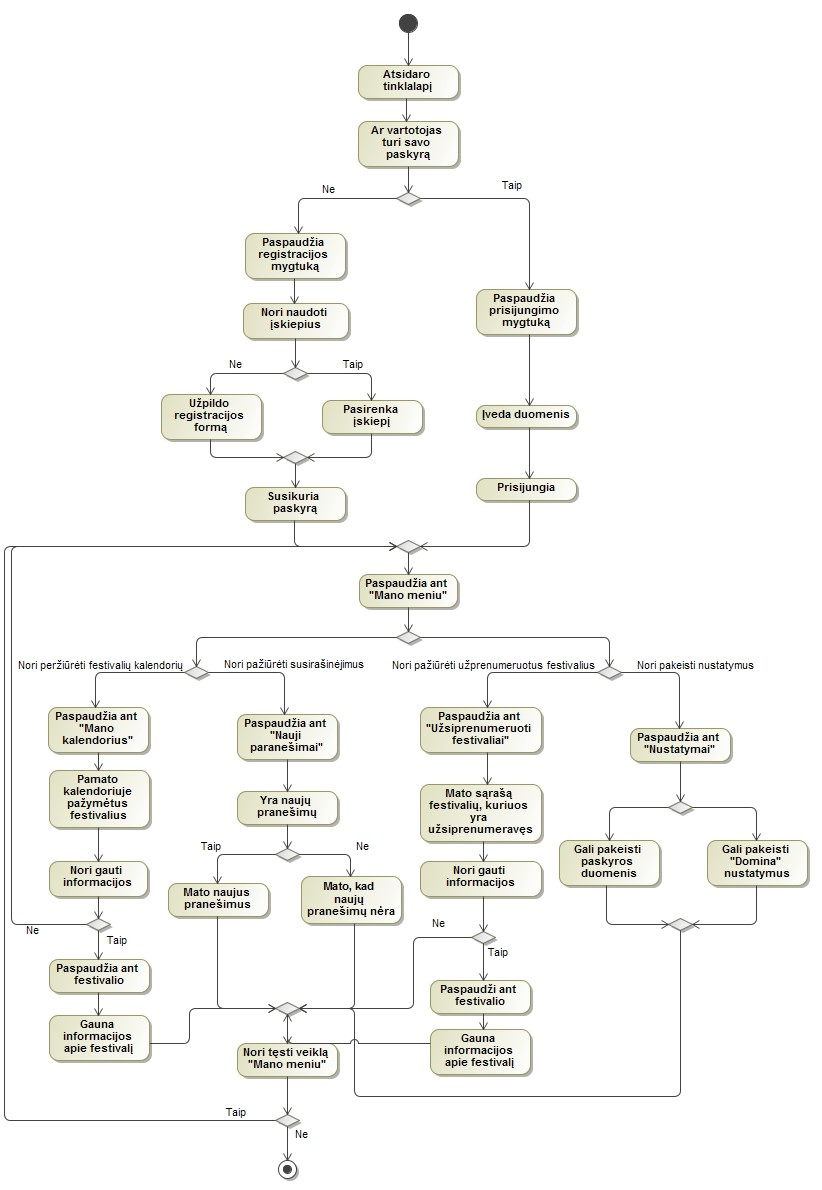
\includegraphics[scale=0.5]{img/Pav/VartotojasPrisijungesFunk}
	\label{uml:24}
	\caption{Vartotojo veiksmai prisijungus}
\end{figure}



\section{Komponentų išskirstymas tinkle}
Pateikiama diegimo diagrama, kurioje pavaizduota, kaip festivalių informacinė sistema bus išskirstyta aparatinėje įrangoje. 
\begin{center}
    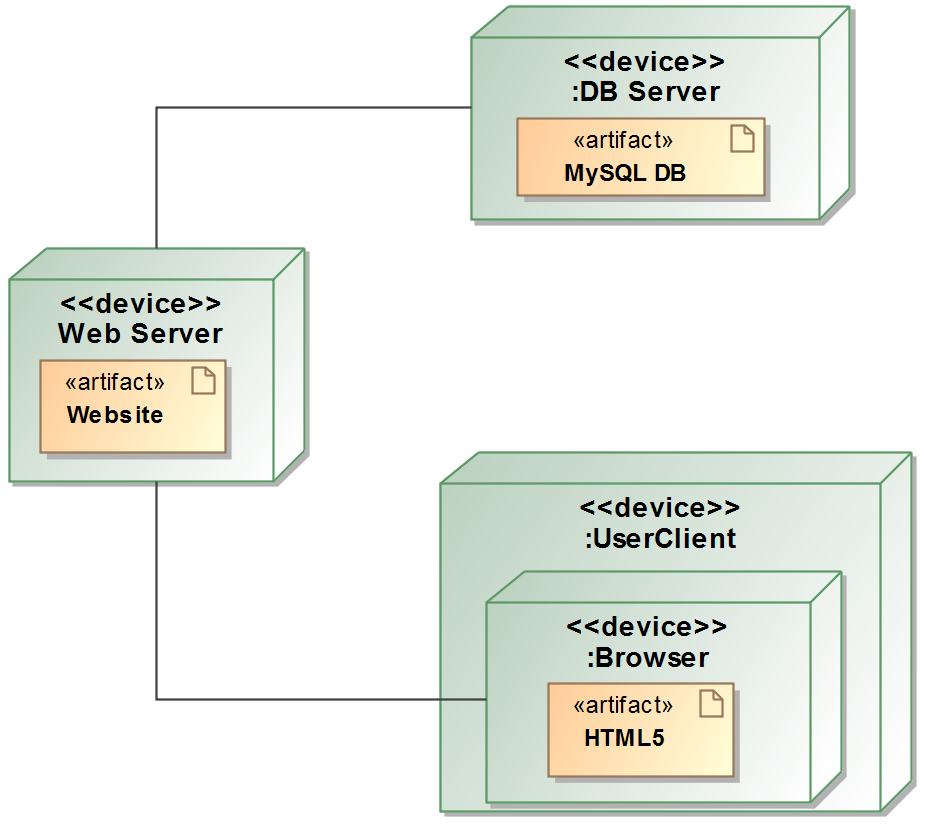
\includegraphics[scale=0.5]{img/PSI3/deploy.PNG}
\end{center}
Informacija yra saugoma duomenų bazės serveryje (\textit{DB Server}), kuriame yra \textit{MySQL} duomenų bazė. Tinklalapis (\textit{Website}), veikiantis žiniatinklio serveryje (\textit{Web Server}), tvarko ir apdoroja informaciją, saugomą duomenų bazėje. Vartotojas pasiekia tinklalapį per naršyklę, palaikančia HTML5. Naršyklę turi būti instaliuota įrenginyje su interneto prieiga.


\section{Verslo proceso aprašas}

Nagrinejama sritis - festivaliu informaciniai šaltiniai. 
Festivaliai yra aktyvi laisvalaikio praleidimo forma, dažnai turi ypatingai didele kulturine verte. 
Festivaliu egzistuoja ivairiausiu tipu (žanru): muzikos, kino, mokslo, poezijos, šokio, teatro, sporto ir dar daugiau. 
Festivaliuose dalyvauja visokio amžiaus ir visokiu pomegiu turintys žmones, taip sukuriantys pakankamai didele paklausa. 
Lietuvoje vasara vyksta daug muzikos festivaliu kaip “Menuo Juodaragis”, “Granatos Live”, “Roko naktys”, “Velnio akmuo”, “Bliuzo naktys” ir daug kitu,
 Lietuvos didžiausias kino festivalis “Kino pavasaris” bei nesuskaiciuojama daugybe ivairiu sporto šaku festivaliu.

Del tokios festivaliu ivairoves negalima visu bendrai apibudinti. Taciau pagrindiniai veiksniai išlieka - festivaliu organizatoriai ir žmones, norintys dalyvauti festivalyje. 
Festivaliu organizatoriai visada siekia reklamuoti savo festivali tam, kad ju renginyje apsilankytu kuo daugiau žmoniu. 
O žmonems reikia patogiai prieinamos informacijos, kad ir taip neturedami laiko, sugebetu susiplanuoti nueiti i keleta renginiu. 
Taciau festivaliu organizatoriai yra linke informacija apie festivalius talpinti savo tinklalapiuose, ir žmonems, norintiems gauti informacijos, reikia aplankyti kiekvieno festivalio tinklalapi atskirai. 
Tai efektyvu ar naudinga nei festivaliu organizatoriams, nei žmonems, kadangi vieni praranda potencialius dalyvius, o kiti praleidžia jiems nežinomus festivalius. 
Šias problemas išsprestu bendra erdve, kurioje festivaliu organizatoriai gales reklamuoti savo festivalius, o žmones gales juos surasti (bei visa informacija apie juos). 
Remdamiesi panašia ideja, 2012 metais grupeleaktyviu festivaliu dalyviu sukure tinklalapi manofestivalis.lt, ju veikla tesiasi iki šiol, o labiau išvystyto tinklalapio Lietuvoje su visa informacija apie festivalius nera. 
Taciau tinklalapiui manofestivalis.lt truksta interaktyvumo su vartotoju, todel, išanalizave ši tinklalapi, mes nusprendeme sukurti patrauklesne alternartyva. 

\vspace{5mm} 

\noindent
Šiuo metu populiariausios sistemos apie festivalius Lietuvoje yra:

\begin{itemize}
\item www.manofestivalis.lt
\item www.isic.lt/vasaros-festivaliai-2016-lietuvoje/
\item www.facebook.com/Festivaliai2015/
\end{itemize}

\noindent
Alternatyvos pasaulyje:

\begin{itemize}
\item www.eventful.com
\item www.fest300.com
\item www.everfest.com
\item www.musicfestivalwizard.com
\end{itemize}

\section{Išorine analize}
Mes analizuosime www.manofestivalis.lt, nes tai yra populiariausia, labiausiai išvystyta ir musu vizijai artimiausia sistema Lietuvoje.
\subsection{"Juodosios dežes" analize}
\begin{figure}[H]
    \centering
    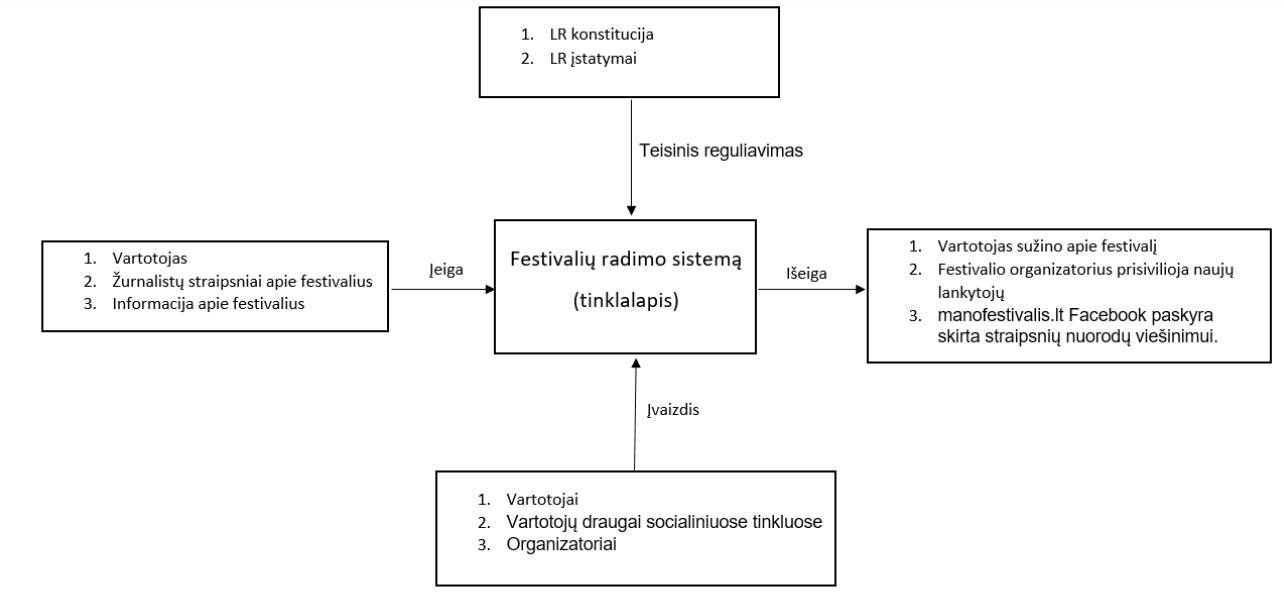
\includegraphics[scale=0.5]{img/geri/IsorineA}
    \label{img:uml0}
	\caption{Ieiga, išeiga ir reguliavimas}
\end{figure}
\noindent
Ieiga:
\begin{itemize}
\item Vartotojas - žmogus isijunges svetaine, norintis gauti informacija, apie buvusius ir ateinancius festivalius;
\item Žurnalistu straipsniai apie festivalius;
\item Informacija apie festivalius - tiekiama festivalio organizatoriu arba surandama administratoriu. Sudedamosios dalys: festivalio tinklalapis, bilietu pardavejas, festivalio vieta, laikas, nuotraukos susijusios su festivaliu(plakatai), festivalio aprašas.
\end{itemize}
Išeiga:
\begin{itemize}
\item Vartotojas sužino apie festivali;
\item Festivalio organizatorius prisivilioja nauju lankytoju;
\item Nuorodos i tinklalapio straipsnius skirtos dalintis “Facebook” paskyroje
\end{itemize}
Ivaizdžio esybes:
\begin{itemize}
\item Vartotojai;
\item Vartotoju draugai socialiniuose tinkluose;
\item Festivaliu organizatoriai
\end{itemize}
Teisinis reguliavimas:
\begin{itemize}
\item Lietuvos Respublikos konstitucija;
\item Lietuvos Respublikos istatymai;
\end{itemize}
\subsection{Aprašas}



“Naujienu” skiltyje klientas mato paveikslelius su straipsniu pavadinimais.
Paspaudus ant ju, pateikiamas straipsnis apie festivali su galimybemis dalintis juo socialiniuose tinkluose ir komentuoti. 

Skiltyje “Festivaliai” yra navigacijos dalis, kurioje galima pasirinkti festivalio kategorija, likusioje skilties dalyje yra paveiksleliu (plakatu), kurie turi festivalio pavadinima bei trumpa informacija apie ji, kratinys. Paspaudus ant paveikslelio, ikeliamas naujas puslapis, kuriame pateikiama informacija apie festivalio vieta (naudojant “Google Maps”), trumpa programa, bilietu kaina, nuorodos i oficialu tinklalapi ir pardaveju puslapi. Yra galimybe pasidalinti informacija apie festivali per “Facebook”, “Google+” ir “Twitter”. Šalia pateikiami naujausiu festivaliu, populiariausiu festivaliu bei panašiu festivaliu sarašai. 

“Kalendoriaus” skiltyje tinklapio lankytojams pateikiamas kalendorius, kuriame festivaliai yra sužymeti pagal dienas.

“Žemelapio”  skiltyje yra pateikiamas “Google Maps” žemelapis, kuriame pažymetos kai kuriu (ne visu) festivaliu vietos bei ju pavadinimai.
 
“Apie mus” skiltyje pateikiama informacija apie tinklapio sukurima, pasiulymas paremti tinklalapi savo 2\% nuo pajamu mokesciu.
Yra atskira skiltis “Pranešk apie festivali”, kuriame lankytojas gali nemokamai pateikti informacija apie festivali nurodydamas pavadinima, kategorija, miesta, tikslu adresa, aprašyma, kaina, festivalio pradžia, pabaiga, festivalio logotipa, oficialu festivalio interneto puslapi, bilietu pirkimo puslapi, kontaktini elektronini pašta. 



\subsection{Metrikos}
\begin{longtable}{|p{0.2\linewidth}|p{0.2\linewidth}|p{0.2\linewidth}|p{0.15\linewidth}|p{0.15\linewidth}|} 
  \caption{Metrikos}\\
	\hline
	Metrikos & Matavimo vienetas & Kaip matuoti & Dabartine reikšme & Kritine reikšme \\
    \hline
    Vartotoju skaicius  & Žmoniu, kurie dažnai naudojasi tinklalapiu, kiekis vienetais   & Suskaiciuoti, kiek žmoniu isijungia tinklalapi nors karta per menesi  & 4 000 & 7 500 \\
	\hline
    Vartotoju aktyvumas  & 
Komentaru ir atsiliepimu, kurie prisideda prie svetaines ir festivaliu informacijos gerinimo, kiekis vienetais
    & Suskaiciuoti, kiek iš viso yra komentaru ir atsiliepimu susijusiu su svetaines veikimu ir tiekiama informacija  & 5 & 1000    \\
    \hline
    “Facebook” puslapio vertinimas žvaigždutemis  & 
Žvaigžduciu kiekis puslapyje
    & Patikrinti žvaigžduciu skaiciu “Facebook” puslapyje  & (nera galimybes apskaiciuoti) & 4,8   \\
    \hline
Tinklalapio peržiuros  & 
Žmoniu, kurie nors karta buvo prisijunge i tinklalapi, kiekis vienetais
    & Suskaiciuoti individualius IP adresus  & 20 000 & 100 000   \\
    \hline
    Žmoniu, potencialiai perkanciu bilieta per nuoroda iš musu puslapio, kiekis   & 
Nuorodos i bilietu tiekejo puslapi paspaudimu kiekis, vienetais 
    & Suskaiciuoti, kiek kartu paspausta nuoroda iš tam tikro festivalio  & (nera galimybes apskaiciuoti) & 10   \\
    \hline
    Atsiliepimu kiekis po festivalio   & 
Po festivaliu aprašymais paliktu komentaru kiekis vienetais 
    & Suskaiciuoti atsiliepimus apie festivali  & 0 & 20   \\
    \hline
    Festivaliu organizatoriu kiekis kurie nori  patalpinti skelbimus   & Organizatoriu, kuriu festivaliu informacija talpiname, kiekis vienetais 
    & Suskaiciuoti visus organizatorius, kurie dalinasi ir trokšta dalintis informacija apie savo organizuojamus festivalius  & 45 & 100   \\
    \hline
    Talpinamu skelbimu kiekis   & 
Skirtingu festivaliu skelbimu kiekis vienetais 
    & Suskaiciuoti kiek iš viso turime skirtingu patalpintu festivaliu  & >2000 & 5000   \\
    \hline 
    Kiekis organizatoriu perkanciu reklama pas mus   & 
Organizatoriu kiekis vienetais
    & Suskaiciuoti kiek organizatoriu perka reklama  & 0 & 16   \\
    \hline
    Kiekis žmoniu, kurie megsta musu puslapi per “Facebook”   &  “Like” kiekis vienetais “Facebook” puslapyje & Patikrinti “Like” skaiciu “Facebook” puslapyje  & 6168 & 50 000   \\
    \hline
    2\% pajamu  mokesciu paramos  kiekis & Vartotoju kiekis kurie skyre 2\% & Peržvelgti kiek vartotoju skyre savo 2\%  & 10 & 100   \\ \hline
\end{longtable}

\section{Vidine proceso analize}
\subsection {Dalykines srities statine struktura}
Išanalizave išorine “manofestivalis.lt” struktura, mes padareme spejima kaip viskas veikia tinklalapio viduje (baltaja deže).
Pagal dalykines srities statine strukura (pav. /?Number?/) matyti pagrindines klases: sistemos savininkas, tinklalapis, festivalio aprašymo puslapis,
 socialiniai iskiepiai (“G+1”, “Tweet”, “Like” mygtukai, “Facebook” komentaru erdve), festivaliu duomenu baze, vartotojas, administratorius, žurnalistas, festivalio organizatorius,
 informacija apie festivali (“Google Maps” žemelapyje pavaizduota festivalio vieta, festivalio data, festivalio nuotraukos, festivalio aprašas, nuorodos i oficialu festivalio tinklalapi bei bilietu pardavimo puslapi). 

\textbf{Tinklalapis} sieja informacija ir vartotojus. Jame talpinami susisteminti festivaliu puslapiai ir straipsniai, leidžiantys vartotojui ieškoti festivaliu. Tinklalapi finansuoja sistemos savininkas, prižiuri ir tvarko sistemos administratorius.

\textbf{Festivalio aprašymo puslapis} talpina socialiniu tinklu iskiepius ir informacija apie festivali, kuria gauna per festivaliu duomenu baze.  

\textbf{Tinklalapio vartotojas} yra informacijos ieškotojas. Jis naudojasi tinklalapiu noredamas sužinoti informacija apie festivalius ir skaityti straipsnius apie festivalius. Jis gali komentuoti apie festivalius ir straipsnius komentaru erdveje prisijunges prie savo “Facebook” paskyros, dalintis informacija naudodamas socialiniu tinklu iskiepius. Taip pat vartotojas gali rašyti atsiliepimus apie pati tinklapi administratoriui.

\textbf{Socialinio tinklalpio iskiepis} leidžia vartotojui reaguoti i pateikta informacija. “Like”, “Tweet”, “G+1” mygtukai  ir “Facebook” komentaru erdve leidžia pasidalinti ar išreikšti savo nuomone, jei jis naudojasi atitinkamo socialinio tinklo paslaugomis.

\textbf{Straipsnio puslapis} yra atskiras puslapis, kuriame bandoma sudominti vartotoja festivaliu. Jis savyje talpina socialinius iskiepius leidžiancius vartotojui vertinti ir dalintis straipsniu.

\textbf{Administratorius} yra pagrindinis tinklalapio veiklos prižiuretojas.
Jis moderuoja komentaru erdve - šalina netinkamus komentarus, prižiuri festivalio organizatoriu pateikiama informacija (ar ši yra teisinga), jei reikia susisiekia su organizatoriumi del papildomos informacijos, užtikrina sklandu puslapio veikima (prižiuri technine tinklalapio dali) ir pats surades festivali, kurio skelbimo dar nera tinklalapyje, gali patalpinti informacija apie ji.

\textbf{Sistemos savininkas} gali sutapti su administrariumi ar žurnalistu arba kitiems paskirti šias pareigas.

\textbf{Festivaliu organizatorius} yra asmuo rengiantis festivali bei turintis oficialia informacija. Noredamas populiarinti savo festivali jis gali pateikti informacija apie savo festivali, kuria ivertines administratorius patalpins tinklalapyje.

\textbf{Žurnalistas} stengiasi populiarinti festivalius ir tinklalapi. Jis gali patalpinti i tinklalapi parašytus ar surastus straipsnius.

\textbf{Festivaliu duomenu baze kaupia} informacija apie festivalius.

\textbf{Informacija apie festivalius} - festivalio aprašymas, data, vieta, kaina, oficialus puslapis ir bilietu pardavejo puslapis (jeigu yra).

\textbf{“Facebook” komentaru erdve} yra socialiniu tinklu iskiepis, kuriame vartotojai gali išsakyti savo mintis naudomi “Facebook” paskyra.

\begin{figure}[H]
    \centering
    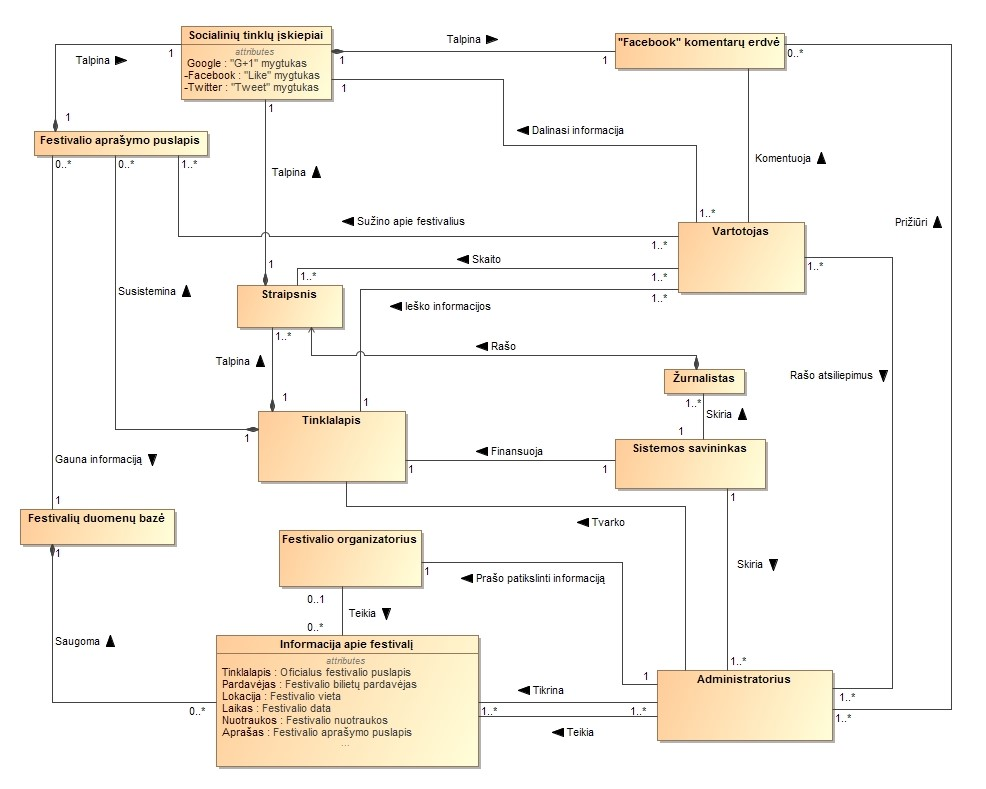
\includegraphics[scale=0.45]{img/geri/Statine_struktura}
    \label{img:uml1}
	\caption{Sistemos statine struktura}
\end{figure}

\subsection {Užduotys}

\begin{figure}[H]
    \centering
    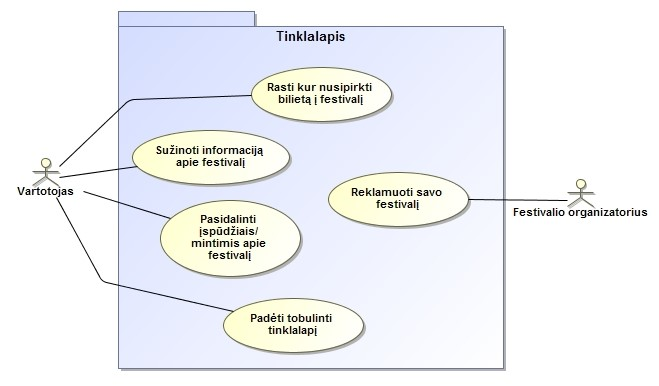
\includegraphics[scale=0.5]{img/geri/UzduotysIS}
    \label{img:uml2}
	\caption{Išoriniu agentu užduotys}
\end{figure}

\begin{itemize}
\item Vartotojas yra agentas, kurio vienas iš siekiu yra ieškoti informacijos apie festivalius (arba tiesiog ieškoti nauju festivaliu, kuriuose galetu sudalyvauti), taciau vartotojas žinodamas, kokiame festivalyje nori dalyvauti jis nebutinai žinos, kur gali nusipirkti bilieta, todel tai yra jo antroji užduotis. Sudalyvave festivalyje arba tiesiog tinklalapio vartotojai gali išsakyti savo nuomone apie pasirinktaji festivali komentaru erdveje. Beje, vartotojas noredamas prisideti prie svetaines gyvavimo bei augimo gali pasidalinti savo idejomis su administratoriumi.
\item Festivalio organizatoriaus pagrindine užduotis yra platinti bei reklamuoti savo festivali tam, kad kuo daugiau žmoniu sudalyvautu jo ruošiamame renginyje.
\end{itemize}

\begin{figure}[H]
    \centering
    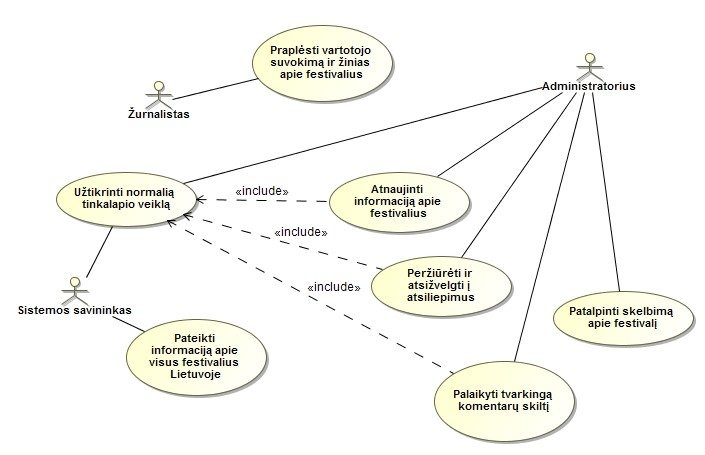
\includegraphics[scale=0.6]{img/geri/UzduotysVID}
    \label{img:uml3}
	\caption{Vidiniu agentu užduotys}
\end{figure}

\begin{itemize}
\item Administratoriaus užduotys kyla iš to, kad jis siekia palaikyti normalia tinklalapio veikla ir augima (nauju festivaliu skelbimu kelima). Tad, administratorius turi prižiureti komentaru erdve tam, kad nebutu netinkamu komentaru (spam, patyciu ir t.t), pasikeitus informacijai apie festivalius ja atnaujinti, kad nebutu apgaulingos (netikslios) reklamos bei atsižvelgti i vartotojo pasiulymus kaip tobulinti svetaines darba, išsidestyma. Taciau vienas iš svarbiausiu užduociu yra kelti naujus skelbimus i tinklalapi, kad jame nuolatos butu aktuali informacija.
\item Sistemos savininkas siekia pateikti lengvai vartotojui prieinama informacija apie visus Lietuvos festivalius viename tinklalapyje, kad jam ieškojimas reikalingos informacijos butu kuo trumpesnis. Beje, sistemos savininkas prižiuri, kad administratorius atliktu savo darba ir tinklalapis veiktu puikiai.
\item Žurnalistas siekia praplesti vartotoju žinias ir suvokima apie festivalius bei sudominti tinklalapio turiniu, nes per straipsnius pristato pagrindine tinklalapio tema - festivalis.
\end{itemize}

\subsection {Užduociu vykdymo scenarijai}

Agentas noredamas atlikti savo užduotis turi atlikti tam tikrus žingsnius.

\subsubsection{Išoriniu agentu užduotys} 
\begin{figure}[H]
    \centering
    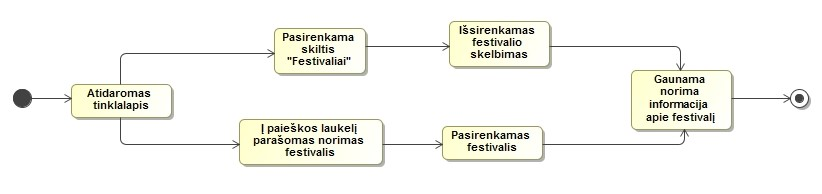
\includegraphics[scale=0.55]{img/geri/klientasInfo}
    \label{img:uml3_5}
	\caption{Vartotojas ieško informacijos}
\end{figure}

Vartotojas noredamas rasti daugiau informacijos:
\begin{itemize}
\item Atidaro tinklalapi.
\item Pirmas atvejis:
\begin{itemize}
\item vartotojas navigacijos dalyje pasirenka skilti “Festivaliai”;
\item festivaliu skelbimu kratinyje išsirenka festivali, apie kuri nori sužinoti daugiau.
\end{itemize}
\item Antras atvejis:
\begin{itemize}
\item i paieškos laukeli ivedamas norimo festivalio pavadinimas;
\item pasirenkamas norimas festivalis.
\end{itemize}
\item Atsidaro naujas tinklalapio puslapis su informacija apie norima festivali.
\end{itemize}

\begin{figure}[H]
    \centering
    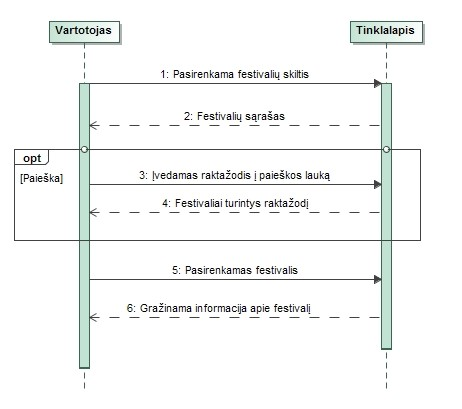
\includegraphics[scale=0.7]{img/geri/_klientasInfo}
    \label{img:uml4}
	\caption{Informacijos gavimo seku diagrama}
\end{figure}

Vartotojas noredamas sužinoti informacija apie festivali, tinklalapyje pasirenka festivaliu skilti. Tinklalapis pateikia festivaliu saraša. Vartotojas gali paieškos laukelyje ivesti norimo festivalio raktažodi ir tinklalapis pateikia tik tuos festivalius, kurie turi ta raktažodi. Arba vartotojas gali iš festivaliu sarašo pasirinkti ji dominanti festivalio skelbima ir tinklalapis gražins informacija apie ji.

\begin{figure}[H]
    \centering
    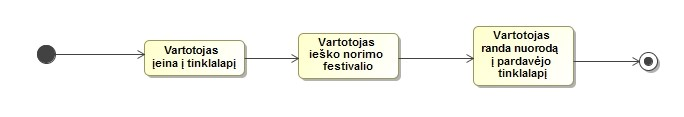
\includegraphics[scale=0.6]{img/geri/klientasBilietas}
    \label{img:uml5}
	\caption{Vartotojas ieško kur nusipirkti bilieta}
\end{figure}

Vartotojas noredamas nusipirkti bilieta i festivali:
\begin{itemize}
\item Atidaro tinklalapi.
\item Randa norima festivali.
\item Festivalio aprašyme randa nuoroda i pardavejo tinklalapi, kuriame isigyja bilieta.
\end{itemize}

\begin{figure}[H]
    \centering
    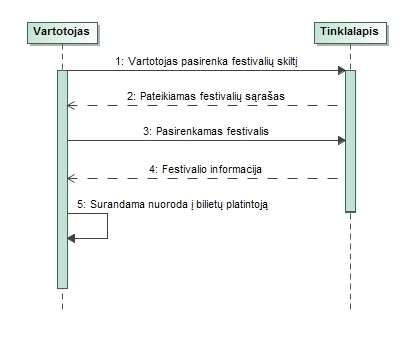
\includegraphics[scale=0.7]{img/geri/_klientasBilietas}
    \label{img:uml6}
	\caption{Bilietu ieškojimo seku diagrama}
\end{figure}

Vartotojas noredamas rasti, kur nusipirkti bilieta, tinklalapyje pasirenka festivaliu skilti. Tinklalapis pateikia festivaliu saraša, iš kurio vartotojas gali pasirinkti norima festivali. Tada tinklalapis vartotojui pateikia festivalio informacija - vartotojas šioje informacijoje suranda nuoroda i bilietu platintoja.

\begin{figure}[H]
    \centering
    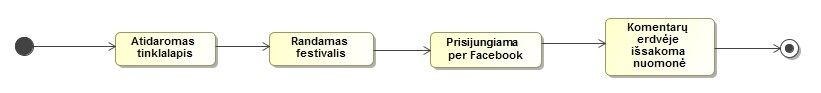
\includegraphics[scale=0.5]{img/geri/klientasmintis}
    \label{img:uml7}
	\caption{Vartotojai komentuoja festivalius}
\end{figure}

Vartotojas noredamas pasidalinti ispudžiais (mintims) apie festivali:
\begin{itemize}
\item Atidaro tinklalapi.
\item Suranda norima festivali.
\item Prisijunges prie “Facebook” paskyros, komentaru erdveje išsako savo nuomone.
\end{itemize}
\begin{figure}[H]
    \centering
    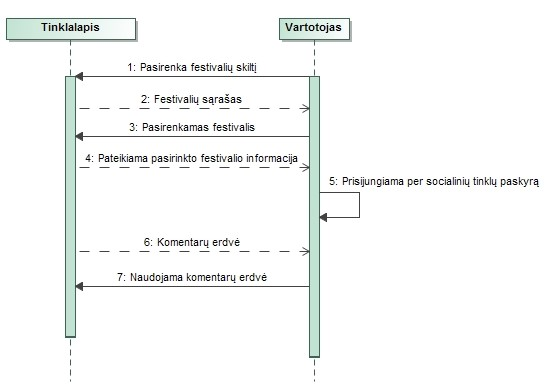
\includegraphics[scale=0.7]{img/geri/_klientasKom}
    \label{img:uml8}
	\caption{Komentavimo seku diagrama}
\end{figure}

Vartotojas noredamas pasidalinti ispudžiais ar mintimis apie festivali gali tinklalapyje pasirinkti festivaliu skilti. Tinklalapis jam pateikia festivaliu saraša, iš kurio vartotojas pasirenka festivali. Tada tinklalapis vartotojui pateikia pasirinktojo festivalio informacija. Vartotojas prisijungia prie savo socialiniu tinklu paskyros ir tada tinklalapis leidžia vartotojui naudotis komentaru erdve.

\begin{figure}[H]
    \centering
    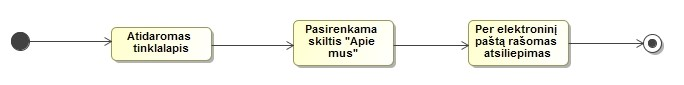
\includegraphics[scale=0.7]{img/geri/klientasKom}
    \label{img:uml9}
	\caption{Vartotojas teikia atsiliepimus}
\end{figure}

Vartotojas noredamas prisideti prie tinklalapio tobulinimo:
\begin{itemize}
\item Atidaro tinklalapi.
\item Navigacijos dalyje pasirenka skilti “Apie mus” bei poskilti “Kontaktai”.
\item Šioje skiltyje randa tinklalapio informacinio elektroninio pašto adresa, kuriuo išsiuncia atsiliepima apie tinklalapi.
\end{itemize}

\begin{figure}[H]
    \centering
    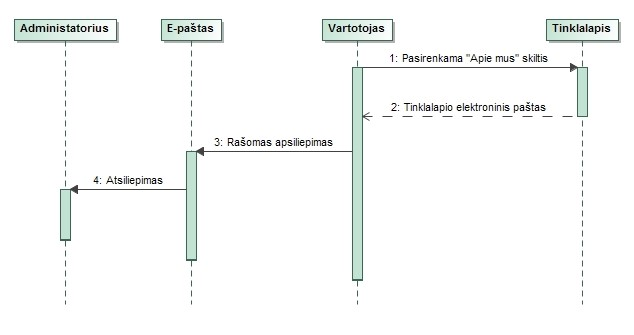
\includegraphics[scale=0.7]{img/geri/_klientasmintis}
    \label{img:uml10}
	\caption{Atsiliepimu seku diagrama}
\end{figure}

Vartotojas noredamas padeti tobulinti tinklalapi , jame pasirenka skilti “Apie mus”, toje skiltyje randa tinklalapio elektronini pašta. Tada vartotojas naudodamasis savo elektroniniu paštu parašo atsiliepima i tinklalapio elektronini pašta. Administratorius gauna elektronini laiška su vartotojo atsiliepimu apie tinklalapi. 

\begin{figure}[H]
    \centering
    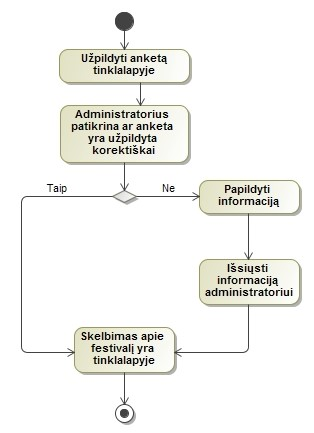
\includegraphics[scale=0.7]{img/geri/festivalOrg}
    \label{img:uml11}
	\caption{Organizatorius nori patalpinti skebima}
\end{figure}

Festivalio organizatorius noredamas reklamuoti savo festivali:
\begin{itemize}
\item Užpildo anketa tinklalapyje.
\item Jei jis gauna puslapio administratoriaus pranešima del netinkamos informacijos, festivalio organizatorius informacija turi patikslinti ir/arba papildyti, nes kitaip administratorius informacijos i tinklalapi neikels.
\end{itemize}

\begin{figure}[H]
    \centering
    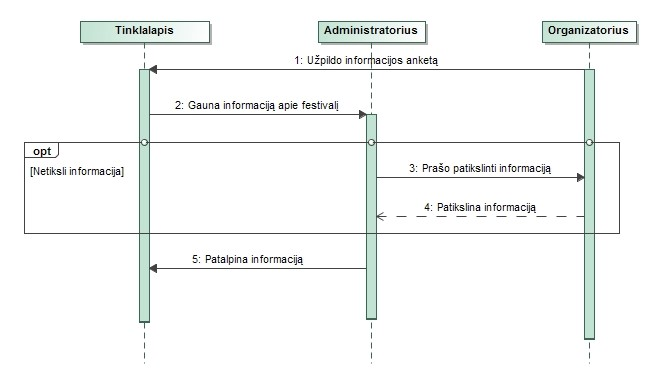
\includegraphics[scale=0.7]{img/geri/_Organizatorius}
    \label{img:uml12}
	\caption{Patalpinimo seku diagrama}
\end{figure}

Festivalio organizatorius tinklalapyje užpildo informacijos anketa. Tada administratorius gauna informacija apie festivali . Jeigu festivalio organizatoriaus informacija yra netiksli arba neteisinga - administratorius parašo ja patikslinti, tuomet festivalio organizatorius patikslina informacija. Ir tada administratorius patalpina informacija (festivalio skelbima) i tinklalapi.

\subsubsection{Vidiniu agentu užduotys} 

\begin{figure}[H]
    \centering
    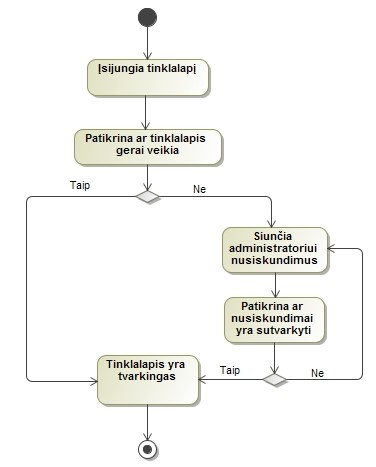
\includegraphics[scale=0.7]{img/geri/sistemosSav}
    \label{img:uml13}
	\caption{Savininkas tikrina tinklalapio tvarkinguma}
\end{figure}

Sistemos savininkas noredamas užtikrinti normalia tinklapio veikla:
\begin{itemize}
\item Ijungia tinklalapi.
\item Tinklalapio veikimo patikrinimas: 
\begin{itemize}
\item tinklalapis greitai (max 5s) pasikrauna, kad vartotojas kuo efektyviau galetu išnaudoti tinklalapi ir kuo daugiau laiko praleistu jame kažka veikdamas, o ne laukdamas, kad pasikraus;
\item tinklalapio informacija turi buti nuolatos atnaujinama ir patikrinama, kad nebutu apgaulingos reklamos ir kad neprarastume vartotojo pasitikejimo tinklalapio informacijos teisingumu;
\item komentaru erdveje nera šlamšto (spam), ižeidžianciu komentaru.
\end{itemize}
\item Jeigu kažkas yra blogai, nusiskundimas yra siunciamas administratoriui: 
\begin{itemize}
\item jis privalo sutvarkyti sistemos savininko nusiskundimus ir tada tinklalapis vel tampa tvarkingu ir normaliai veikianciu;
\item jeigu ne - sistemos savininkas patikslina savo nusiskundima tam, kad adminsitratorius geriau suvoktu, ka reikia pakeisti ar pataisyti.
\end{itemize}
\end{itemize}

\begin{figure}[H]
    \centering
    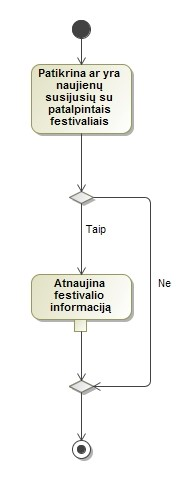
\includegraphics[scale=0.7]{img/geri/adminAtnaujinti}
    \label{img:uml14}
	\caption{Administratorius atnaujina fesitvalio informacija}
\end{figure}

Administratorius, noredamas atnaujinti informacija apie festivali:
\begin{itemize}
\item Suranda patikimu naujienu apie festivalius, kuriu informacija jau patalpinta tinklalapyje, arba festivalio organizatorius praneša apie pakitusia festivalio informacija.
\item Jeigu yra pakitus festivalio informacija, ja atnaujina, kad vartotojas galetu rasti tik tikslia informacija.  
\end{itemize}

\begin{figure}[H]
    \centering
    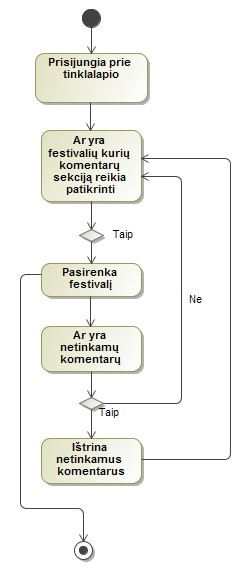
\includegraphics[scale=0.7]{img/geri/adminKom}
    \label{img:uml15}
	\caption{Administratorius palaiko tvarkinga komentaru skilti}
\end{figure}

Administratorius, noredamas palaikyti tvarkinga komentaru skilti:
\begin{itemize}
\item Prisijungia prie tinklalapio.
\item Patikrina ar yra netikrintu festivaliu komentaru sekciju:
\begin{itemize}
\item Jeigu yra, pasirenka festivali;
\item Patikrina ar yra netinkamu komentaru:
\begin{itemize}
\item Patyciu,
\item Diskriminacijos,
\item Neatitinkanciu temos,
\item Prieštarajanciu Lietuvos istatymams ir “Facebook” taisyklems.
\end{itemize}
\item Pašalina netinkamus komentarus.	
\end{itemize}
\end{itemize}

\begin{figure}[H]
    \centering
    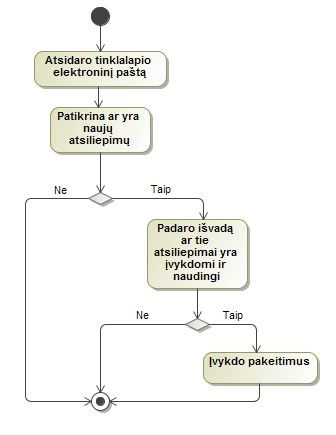
\includegraphics[scale=0.7]{img/geri/adminFeed}
    \label{img:uml15_5}
	\caption{Administratorius peržiuri atsiliepimus}
\end{figure}

Administratorius noredamas peržiureti vartotoju atsiustus atsiliepimus:
\begin{itemize}
\item Atsidaro informacini tinklalapio elektronini pašta.
\item Patikrina ar yra nauju atsiliepimu iš vartotoju.
\item Jeigu yra nauju, tuomet:
\begin{itemize}
\item Ivertina ar atsiliepimai yra naudingi tinklalapiui ir ar pasiulymai yra ivykdomi;
\item Jeigu taip, ivykdo pakeitimus.
\end{itemize}
\end{itemize}

\begin{figure}[H]
    \centering
    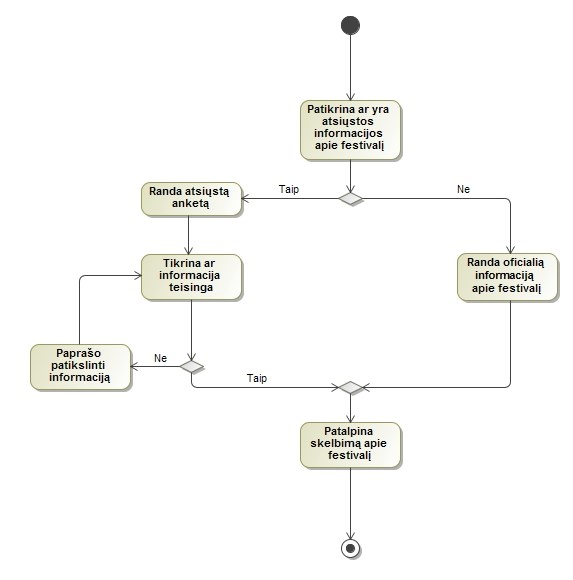
\includegraphics[scale=0.7]{img/geri/adminSkelb}
    \label{img:uml16}
	\caption{Administratorius ikelia skelbima i FDB}
\end{figure}

Administratorius noredamas patalpinti i FDB nauja skelbima apie festivali:
\begin{itemize}
\item Prisijungia prie FDB.
\item Jei yra pateikta nauja arba patikslinta informacija apie festivalius:
\begin{itemize}
\item Tikrina ar informacija yra teisinga.
\item Jeigu informacija netinkama, prašo festivalio organizatoriaus patikslinti informacija.
\item Jeigu informacija teisinga, patalpina skelbima apie festivali i tinklalapi.
\end{itemize}
\item Jei naujos informacijos nepateikta:
\begin{itemize}
\item Ieško naujos informacijos.
\item Rasta informacija, talpina i tinklalapi.
\end{itemize}
\end{itemize}

\begin{figure}[H]
    \centering
    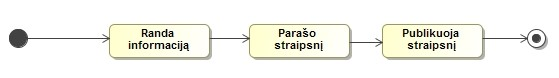
\includegraphics[scale=0.7]{img/geri/zurnalistas}
    \label{img:uml17}
	\caption{Žurnalistas publikuoja straipsni}
\end{figure}

Žurnalistas noredamas praplesti vartotojo žinias ir suvokima apie festivalius:
\begin{itemize}
\item Randa informacija apie festivalius.
\item Parašo straipsni remdamasis rasta informacija.
\item Publikuoja straipsni i tinklalapi.
\end{itemize}

\subsection{Dalykines srities dinamine struktura}
\begin{figure}[H]
    \centering
    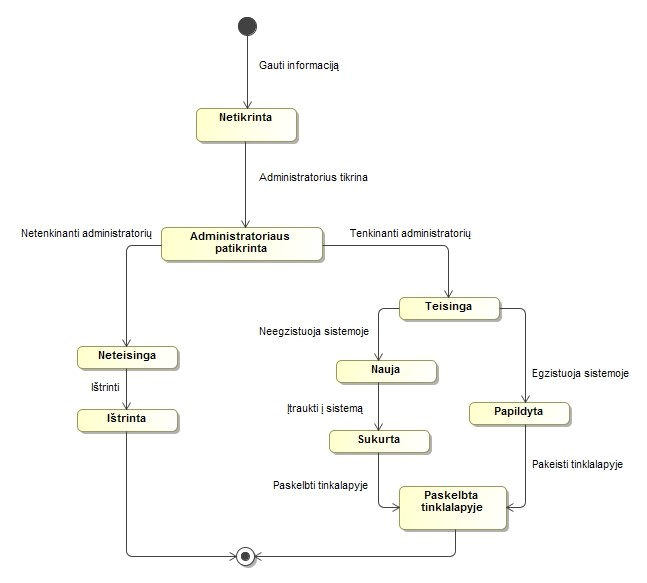
\includegraphics[scale=0.7]{img/geri/Informacija_Busenos.jpg}
    \label{img:uml18}
	\caption{Festivalio informacijos busenos}
\end{figure}
Informacija apie festivalius gali buti ivairiu busenu: netikrinta, administratoriaus patikrinta, teisinga, neteisinga, nauja, sukurta, papildyta, paskelbta tinklalapyje, ištrinta. Kai festivalio organizatorius užpildo tinklalapyje esancia anketa, ji yra gaunama i informacija apie festivalius dali ir turi busena netikrinta. Kai administratorius patikrina informacija apie festivali, ji igauna busena administratoriaus patikrinta. Po patikrinimo informacija gali:
\begin{itemize}
\item netenkinti administratoriaus (šlamštas, reklama, nepagarba kitiems ir t.t.) ir tureti busena neteisinga, o po to, buna ištrinama ir taip igauna busena ištrinta;
\item tenkinti administratoriu ir tureti busena teisinga. Festivalio skelbimas gali jau egzistuoti sistemoje, bet nebuti paskelbtas del to, kad yra reikalingas papildymas ir ši nauja informacija yra jau esancio festivalio informacijos papildymas ir taip informacija apie festivalius igauna busena papildyta. Taciau informacijos gali ir nebuti sistemoje todel ji igauna busena nauja. Ir administratoriui itraukus ja i sistema ji gauna busena sukurta. 
\end{itemize}
Abiem atvejais informacija apie festivalius (ar papildyta, ar sukurta) pasiekia busena paskelbta tinklalapyje.

\begin{figure}[H]
    \centering
    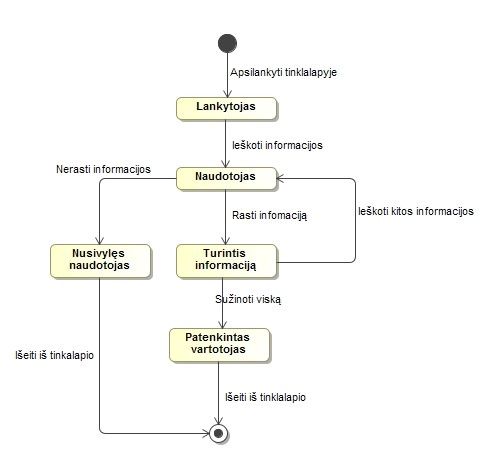
\includegraphics[scale=0.7]{img/geri/Vartotojas_Busenos.jpg}
    \label{img:uml19}
	\caption{Vartotojo busenos}
\end{figure}
Vartotojas gali buti: lankytojas; naudotojas; naudotojas, turintis informacija; nusivyles naudotojas; patenkintas vartotojas. Kai vartotojas apsilanko tinklalapyje jis gauna busena lankytojas. Bet kai vartotojas ne vien apsilanko, bet ir ieško informacijos, jis tampa naudotoju. Nerades jam reikalingos informacijos naudotojas igauna busena nusivyles naudotojas. Kai naudotojas randa informacija jis tampa turintis informacija, bet jei jis nerado visos jam reikiamos informacijos jis gali toliau ieškoti ir vel tampa naudotoju. Jeigu naudotojas randa visa jam norima informacija jis igauna busena patenkintas vartotojas.

\begin{figure}[H]
    \centering
    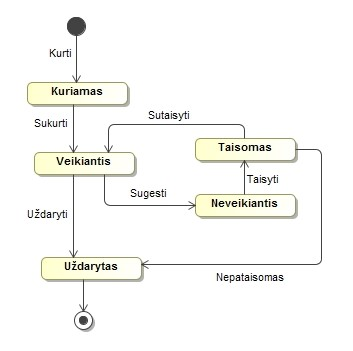
\includegraphics[scale=0.8]{img/geri/Tinkalalio_Busenos.jpg}
    \label{img:uml20}
	\caption{Tinkalalio busenos}
\end{figure}
Tinklalapis gali buti: kuriamas, veikiantis, neveikiantis, taisomas, uždarytas. Jeigu tinklalapis neveikia del serverio talpintoju problemu arba del sistemos klaidu jis igauna busena neveikiantis. Pradejus taisyti neveikiantis tinklalapis tampa taisomu. Pavykus sutaisyti tinklalapis grižta i normalia busena - veikiantis. Del finansu stygiaus arba populiarumo stygiaus tinklalapis gali tapti uždarytu.

\section{Analizes rezultatai}
\begin{longtable}{|p{0.45\linewidth}|p{0.45\linewidth}|} 
  \caption{SSGG}\\
  \hline
  \textbf{Stiprybes}
  \begin{itemize}
	\item Yra informatyviausias tinklalapis apie festivalius Lietuvoje.
	\item Festivaliu organizatoriai gali laisvai reklamuoti renginius. Virš 6100 žmoniu yra pamege "manofestivalis.lt".
	\item Festivaliai turi lygias galimybes - jie rodomi taip pat, neatsižvelgiant i ju populiaruma.
  \end{itemize}
  &
  \textbf{Silpnybes}
  \begin{itemize}
	\item Festivaliu skelbimai pateikiami kaip neorganizuotas paveiksleliu kratinys.
	\item Pasene festivaliu skelbimai nera išimami iš bendros ateinanciu festivaliu erdves, todel vartotojui yra sukuriama iliuzija, kad Lietuvoje atitinkamu metu vyksta daug festivaliu.
	\item Festivaliu ieškojimas yra neefektyvus del per didelio skaiciaus senu festivaliu.
	\item Vartotojai beveik nesinaudoja komentaru erdve. Net didžiausi Lietuvos festivaliai susilaukia tik po viena komentara.
	\item Administratorius nebutinai tinkamai atlieka savo darba, kadangi sistemos savininkas ne visa laika ji kontroliuoja.
	\item Festivaliu skelbimas gali buti patalpintas tinklalapio administratoriaus be festivalio organizatorius žinios.
	\item Festivaliu organizatoriai tinklalapio nemato kaip tikslingos vietos reklamuotis del per mažo populiarumo.
	\item Tinklalapis negeneruoja lešu.
  \end{itemize}\\
  \hline
  \textbf{Galimybes}
  \begin{itemize}
	\item Sukurti vartotojui patogia festivaliu rikiavimo ir rušiavimo sistema pagal data, kaina, miesta, kad vartotojas lengvai pasiektu reikalinga informacija.
	\item Platesnis tinklalapio interaktyvumas - žmones gales patogiau išreikšti savo nuomone ir planuotis i kokius festivalius nori nueiti.
	\item Patobulinti komentaru erdve, kad žmones galetu lengviau susipažinti su kitais festivaliu dalyviais.
	\item Festivaliai galetu išsipirkti savo  skelbimams specialias galimybes taip remdami tinklalapio pletimasi.
	\item Sukurti marketingo komanda, kuri siektu išpopuliarinti tinklalapi tam, kad festivaliu organizatoriai noretu deti savo skelbimus i tinklalapi.
  \end{itemize}
  &
  \textbf{Gresmes}
  \begin{itemize}
	\item Tinklalapio išlaikymas priklauso nuo vartotoju noro skirti savo lešas.
	\item Del didelio senu festivaliu kiekio festivaliai gali netilpti duomenu bazeje.
	\item Kiti tinklalapiai gali aplenkti savo populiarumu ir ryšiais su organizatoriais.
	\item Serveris gali neatlaikyti lankytoju skaiciu.
	\item Del musu tinklalapyje naudojamu socialiniu tinklu iskiepiu mes prarandame komentaru ir vertimu kontrole. / Sklandus vertinimu ir komentaru erdves veikimas yra priklausomas nuo socialiniu tinklu veikimo.
  \end{itemize}\\
  \hline
\end{longtable}

\section{Verslo proceso tobulinimo strategija}
Pagrindinis musu tikslas yra sukurti geresne sistema negu, kad jau yra sukurta. Šito mes sieksime padidindami tinklalapio interaktyvuma (vartotojas gales susikurti paskyra, o prisijunges tures daugiau galimybiu (pateikta žemiau), palengvinsime festivaliu paieška), populiarinti tinklalapi Lietuvos mastu (stengtis, kad daugiau Lietuvos gyventoju žinotu bei naudotusi tinklalapiu, festivaliu organizatoriai siektu reklamuotis tinklalapyje), sukursime galimybe tinklalapiui finansuoti save, palengvinsime tinklalapio administratoriaus darba.

Musu vizija yra padidinti žmoniu aktyvuma bei kulturini suvokima.
Musu misija yra palengvinti festivaliu informacijos pasiekiamuma bei suprantamuma.
\begin{itemize}
\item Paskatinti vartotoja sugrižti i svetaine:
	\begin{itemize}
    \item Padaryti galimybe vartotojui susikurti paskyra tinklalapyje arba prisijungti su turima socialiniu tinklu paskyra (“G+”, “Facebook”) ;
    \item Vartotojas susikures paskyra galetu:
        \begin{itemize}
        \item kalendoriuje pasižymeti festivalius, kuriuose nori sudalyvauti;
        \item užsiprenumeruoti festivaliu skelbimus (jeigu festivalio informacija yra atnaujinama vartotojas bus perspejamas);
        \item likus 3 dienoms iki festivalio vartotojas, jeigu yra pasižymejes kalendoriuje arba užsiprenumeraves, butu perspetas apie meteorologines salygas festivalio dienomis;
        \item vartotojai norintys dalyvauti tame paciame festivalyje galetu tarpusavyje bendrauti atskiroje diskusiju erdveje;
        \item rašyti atsiliepimus apie festivalius tam skirtoje tinklalapio erdveje;
        \end{itemize}
    \end{itemize}
\item Patobulinti tinklalapio festivaliu skiti:
    \begin{itemize}
    \item Leisti vartotojui pasirinkti kokius festivalius jis nori matyti: busimus, vykstancius, praejusius ar visus;
    \item Padaryti galimybe vartotojui pasirinkti pagal kokius kriterijus (datos intervala, miesta, kainos intervala) rušiuoti festivalius, pasirinkti rikiavima pagal pavadinima, data;
    \item Suvienodinti festivaliu skelbimu dydi ir automatiškai surikiuoti chronologine tvarka;
    \end{itemize}
\item Sukurti galimybe tinklalapiui išlaikyti paciam save:
    \begin{itemize}
    \item Kai kurias tinklalapio dalis paskirti mokamai festivaliu reklamai (ju reklamos bus rodomos paskirtose tinklalapio dalyse iki išpirkto laiko pabaigos, ne vien festivaliu skiltyje);
    \end{itemize}
\item Paskatinti vartotojus naudotis komentaru erdve:
    \begin{itemize}
    \item Pašalinti “Facebook” komentaru erdve;
    \item Sukurti tinklalapio komentaru erdve, kurioje prisijunge vartotojai galetu komentuoti apie festivali;
    \item Prisijungusiems tinklalapio vartotojams sukurti atskira diskusiju erdve bendrauti tarpusavyje apie festivalius, kuriuose dalyvaus;
    \end{itemize}
\item Didinti tinklalapio populiaruma:
    \begin{itemize}
    \item Sukurti marketingo komanda, kuri tiesiogiai susisiektu su festivaliu organizatoriais ir pasiulytu patalpinti ju skelbima musu sistemoje, bendrautu del galimu bendru akciju;
    \item Marketingo komanda stengiasi sukurti bendruomene “Facebook” tinklapyje ir taip paskatinti vartotojus naudotis tinklalapiu;
    \end{itemize}
\item Supaprastinti administratorius darba:
    \begin{itemize}
    \item Sukurti “Admin panel” kuriame galima butu matyti po praejusio tikrinimo atsiradusius komentarus;
    \item Leisti vartotojams pranešti apie netinkamus komentarus ar netikslia informacija;
    \end{itemize}
\end{itemize}

\section{Sistemos naudojimo scenarijus}
\subsection{Scenarijus}

Administratorius gali buti perspetas del netinkamu komentaru bei matyti naujus komentarus.

\begin{figure}[H]
    \centering
    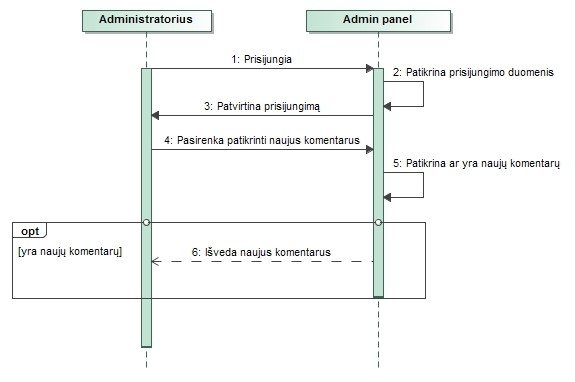
\includegraphics[scale=0.7]{img/geri/_adminNaujiCom}
    \label{img:uml21}
	\caption{"Admin panel" naudojimo seku diagrama}
\end{figure}

Administratorius, noredamas patikrinti komentarus, tures prisijungti prie “Admin panel” (jei prisijungimo duomenys teisingi, patvirtina prisijungima), tada “Admin panel” išveda naujus komentarus administratoriui, o jis juos patikrina.

\begin{figure}[H]
    \centering
    \includegraphics[scale=0.7]{img/geri/_adminError}
    \label{img:uml22}
	\caption{Netinkamos informacijos šalinimo seku diagrama}
\end{figure}

Kad butu lengviau surasti netinkama informacija tinklapyje, vartotojas gales administratoriui apie tai pranešti. Vartotojas, rades klaidingos informacijos festivaliu skiltyje, praneša apie klaida naudodamas tam skirta funkcija ir automatiškai gauna žinute su padeka. Pranešimas apie klaida yra nusiunciamas administratoriui, jis patikrina informacija festivaliu skiltyje ir, jeigu yra klaida, ja ištaiso.

Vartotojas yra dvieju busenu: turintis tinklalapio paskyra arba ne. Nuo to priklauso, kaip jis saveikauja su sistema. 

\begin{figure}[H]
    \centering
    \includegraphics[scale=0.7]{img/geri/KlientPaieska}
    \label{img:uml23}
	\caption{Festivaliu detalesnes paieškos seku diagrama}
\end{figure}

Vartotojas, neturintis paskyros, gali ieškoti informacijos. Festivaliu skiltis pateikia chronologiškai išrikiuotus festivaliu skelbimus bei detalesnes paieškos meniu. Vartotojas, norintis ieškoti tam tikru festivaliu, gali pasirinkti rušiavimo kriterijus (datos intervala, miesta, kainos intervala) bei pakeisti rikiavimo kriteriju (pagal pavadinima arba data). Festivaliu skiltis gražina saraša, išrušiuota ir išrikiuota pagal vartotojo pageidavimus.

\begin{figure}[H]
    \centering
    \includegraphics[scale=0.5]{img/geri/KlientPrisijungimas}
    \label{img:uml24}
	\caption{Vartotojo prisijungimo ir registracijos seku diagrama}
\end{figure}

Vartotojas, noredamas prisijungti prie tinklalapio, gali tai padaryti naudodamasis socialiniais tinklais (“G+”, “Facebook”). Tinklalapyje vartotojas pasirenka šia galimybe, iš tinklalapio yra nukreipiamas i socialinius tinklus ir indentifikuojamas. Tada tinklalapis rodo vartotojo meniu. Taciau vartotojas gali prisijungti prie tinklalapio ir per vietine paskyra. Jeigu vartotojas neturi vietines paskyros, pasirenka ja sukurti ir suveda visus reikiamus duomenis. Sistema patikrina ar toks vartotojas jau yra. Jeigu yra - išspausdina, kad toks vartotojas jau egzistuoja, jeigu ne - praneša, kad registracija sekminga. Jei vartotojas jau turi paskyra ir tiesiog nori prisijungti, suveda savo prisijungimo duomenis. Sistema patikrina, ar duomenys yra teisingi. Jeigu duomenys yra neteisingi, tinklalapis praneša, kad prisijungimo duomenys neteisingi. Jeigu teisingi, atidaro vartotojo meniu.

\begin{figure}[H]
    \centering
    \includegraphics[scale=0.5]{img/geri/KlientFun}
    \label{img:uml25}
	\caption{Vartotojo galimybiu seku diagrama}
\end{figure}

Prisijungusiam vartotojui  tinklalapis rodo vartotojo meniu. Vartotojas kalendoriuje gali pažymeti, kad dalyvaus festivalyje: pasirenka festivali, tinklalapis atidaro festivalio puslapi musu tinklalapyje. Kai vartotojas pasirenka “Dalyvausiu”, kalendoriuje pažymimos dienos, kuriomis vyks festivalis. Ivykdes užduoti tinklalapis praneša vartotojui, kad festivalis pasirinktas. Jei vartotojas pasirenka “Domina”, tinklalapis praneša, kad festivalis yra sekmingai užprenumeruotas. Vartotojas taip pat gali peržiureti savo kalendoriu, kuriame jis yra pažymejes, kuriuose festivaliuose nori dalyvauti arba dalyvaus. Likus trims dienoms iki festivaliu, kuriuos vartotojas yra pasižymejes kalendoriuje arba užsiprenumeraves, vartotojas elektroniniu laišku yra perspejamas apie meteorologine situacija festivalio vietoje. Vartotojas, tinklapyje pasirinkes festivali, gali patekti i diskusijos puslapi ir dalyvauti diskusijoje. Vartotojas gales rašyti naujus pranešimus ir tinklalapis juos saugos. Vartotojas yra perspejamas, kai po jo pranešimu kitas vartotojas parašo komentara. Atidares festivalio puslapi, registruotas vartotojas mato komentaru sekcija, kurioje gali reikšti savo nuomone apie festivali. Tinklalapis išsaugo komentarus sistemoje.

Marketingo komanda gali susisiekti su festivaliu organizatoriais ir jiems pasiulyti reklamuotis musu tinklalapyje bei per socialinius tinklalapius skelbti savo tinklalapi.

\begin{figure}[H]
    \centering
    \includegraphics[scale=0.5]{img/geri/markfacebook}
    \label{img:uml26}
	\caption{Marketingo komandos reklamavimo seku diagrama}
\end{figure}

Marketingo komanda noredama rasti nauju vartotoju, kelia musu tinklalapio straipsniu nuorodas i socialinius tinklus, šias nuorodas randa socialiniu tinklu vartotojai. Jie jas atsidaro ir ieina i tinklalapi.

\begin{figure}[H]
    \centering
    \includegraphics[scale=0.7]{img/geri/markIesko}
    \label{img:uml27}
	\caption{Susiekimo su orgamizatoriais seku diagrama}
\end{figure}

Marketingo komanda, noredama pasiulyti festivaliu organizatoriams skelbtis musu tinklalapyje, susisiekia su festivaliu organizatoriais ir pasiulo reklamuotis tinklalapyje. Jeigu festivalio organizatorius sutinka, marketingo komanda užduoda klausimus festivalio organizatoriui, kad surinktu visa reikiama informacija anketai užpildyti. Marketingo komanda atidaro sistema ir pasirenka naujo skelbimo anketa, ja užpildo. Jei visi duomenys yra korektiški, festivalio skelbimas patalpinamas i tinklalapi.

\subsection{Sistemos teikiama nauda}

\begin{figure}[H]
    \centering
    \includegraphics[scale=0.5]{img/geri/sisNauda}
    \label{img:uml28}
	\caption{Sistemos teikiamos naudos diagrama}
\end{figure}

\subsection{Esama bukle}
\begin{itemize}
	\item 4 kompiuteriai
	\item 4 žmones
\end{itemize}

\subsection{Priemones scenarijui igyvendinti}
\begin{itemize}
\item Serverio nuoma - tinklapio talpinimui, del padidejusio lankytoju skaiciaus senas serveris gali buti netinkamas;
\item Duomenu baze - talpinama informacija apie fesitvalius, vartotoju informacija (prisijungimo duomenys, komentarai ir pan.), straipsnius.
\item “Microsoft Office” licencija - straipsniu rašymui ir buhalterijos vedimui;
\item “Photoshop” licencija - i tinklapi keliamu nuotrauku redagavimui;
\item Verslo liudijimas - legaliam reklamos erdves tinklapyje pardavimui;
\item Facebook reklamos - sistemos populiarinimui;
\item Žmogiškieji ištekliai:
    \begin{itemize}
    \item Programuotoju paslaugos - nauju funkciju kurimui ir diegimui;
    \item Marketingo komanda - sistemos populiarinimui, komunikacijai su festivaliu organizatoriais;
    \item Administratoriai - sistemos tvarkai palaikyti;
    \item Žurnalistas - straipsniu rašymui.
    \end{itemize}
\end{itemize}

\section{Igyvendinamumo ir naudos analize}
\subsection{Operacinis igyvendinamumas}
\begin{longtable}{|p{0,45\linewidth}|p{0,45\linewidth}|}
\caption{Operacinis igyvendinamumas}\\
	\hline
	Inovacinis slenkstis & Inovacinio slenkscio pašalinimas\\
	\hline
	Festivaliu informacine sistema nera žinoma tarp potencialiu lankytoju. &
	Reklamuoti socialiniuose tinkluose.\\
	\hline
	Lankytojai nežino visu tinklalapio galimybiu ir kaip jomis naudotis. &
	Informuoti lankytojus. Užsiregistravusiems vartotojams, kartu su registracijos patvirtinimu, i elektronini pašta atsiusti detalu visu galimybiu aprašyma bei kaip jomis pasinaudoti. Sukurti vartotojui lengvai suprantama vartotojo sasaja. Puslapyje pateikti informacini elektroninio pašto adresa ir atsakyti i vartotojams kylancius klausimus.\\
	\hline
	Festivaliu informacine sistema nera žinoma tarp festivaliu organizatoriu. & Susisiekti su festivaliu organizatoriais.\\
	\hline
\end{longtable}
\subsection{Techninis igyvendinamumas}
Musu kuriama sistema nera visiškai nauja ideja. Analizes metu mes apžvelgeme panašia egzistuojancia sistema, taciau musu sistema butu labiau išbaigta ir turetu daugiau funkciju. Sistemos funkcijoms igyvendinti reikia tinklalapio ir duomenu bazes, kurie galetu buti patalpinti viename serveryje. Duomenu bazeje lentelese butu talpinama informacija apie festivali, komentarus ir vartotoju informacija.

Susikurdami tinklalapio paskyra vartotojai tures užpildyti paskyros laukelius, o prisijungdami per socialinius tinklus už vartoja bus pasirupinta tu laukeliu užpildimu ir naujos paskyros tinklalapyje sukurimu.
\subsection{Ekonominis igyvendinamumas}
\subsubsection{Išlaidos}
 
Musu tinklalapis talpins informacija apie festivali, todel mums reikes serverio ir domeno. Serverio kainos svyruoja nuo 1€ iki 30€, domena galima nusipirkti už 8€ .
Musu tinklalapi aptarnaujancia komanda sudaro administratoriai, žurnalistai ir marketingo komanda. Tiketina, kad menesinis atlyginimas administratoriui sieks 600€ (+ 240€ mokesciu),  žurnalistui ir marketingo komandos nariui po 400 (+160€). Tikriausiai turesime po viena kiekvienos komandos nari.  Norint išpopuliarinti tinklalapi, reiketu užsakyti reklama “Facebook” tinke. Per diena ketiname išleisti apie 10€ reklamai. Tinklalapi kuriantiems programuotojams moketumeme 1500€, tikedamiesi kad jie pilnai sukurs sistema per 3 menesius.
 
Pradines išlaidos: 4500€
 
Menesines išlaidos: 2038€ (1400€ atlyginimas + 560€ mokesciai +60€ reklama +18€ tinklalapio išlaikymas)
 
\subsubsection{Pajamos}
 
Musu tinklalapis pajamas generuos parduodamas išskirtine reklama festivaliu organizatoriams ir prašydamas vartotoju skirti 2\% nuo pajamu mokesciu. Tiketina kad reklama pirmuoju laikotarpiu kainuos 30€ /men ir turesim tik viena reklamos pirkeja. Tinklalapiui išpopuliarejus kaina pakils iki 10€ / dienai ir turesime 3 reklamos pirkejus. 2\% mokesciu nuo vidutinio darbo užmokescio siekia apie 3,5€. Pradžioje planuojame tureti 5 paramos skyrejus, o išpopuliarejus - apie 100 skyreju.
 
Menesines pajamos:
 
Pradejus veikla: 45€
 
Išpopuliarejus: 1250€
 
Mes sieksime gauti Europos sajungos finansavima. Galvojame pateikti užklausa projektui - Ekologinio (pažintinio) turizmo, aktyvaus poilsio ir sveikatos gerinimo infrastrukturos kurimas ir pletra. Mes teigtume, kad musu tinklalapis, turedamas visa reikalinga informacija apie festivalius Lietuvoje, paskatins žmones aktyviai praleisti savo laisvalaiki ir ilgalaikiu požiuriu gali pritraukti turistus i Lietuva del kulturiniu ir kokybišku festivaliu. Tai gali padidinti miestu, kuriuose vyksta festivaliai, iplaukas.
\subsection{Juridinis Igyvendinamumas}
 Musu kuriamai sistemai svarbiausias juridinis klausimas yra - ar nebus pažeistas asmens duomenu teisines apsaugos istatymas. Musu sistemos funkcionalumas ir tikslai nepažeidžia asmens duomenu apsaugos istatymo tikslo - “ginti žmogaus privataus gyvenimo nelieciamumo teise tvarkant asmens duomenis”. Musu sistema registracijos metu prašo tik susisiekimui reikalingu duomenu (elektroninio pašto) ir vartotojui kuriantis paskyra bus prašoma ivesti jo paties sugalvota slapyvardi, kuris bus naudojamas jo identifikacijai, taip nuslepiant jo tikraja tapatybe. Iš socialiniu tinklu (jeigu vartotojas nuspres registruotis per juos) tinklalapis ims tik paskyrai sukurti reikalinga informacija.
%\printbibliography[heading=bibintoc] 
\section{Žodynas}
\begin{sortedlist}
  \sortitem{Sistemos savininkas - fizinis arba juridnis asmuo, kuriam priklauso turtas (tinklalapis).}
  \sortitem{Tinklalapis - informacijos šaltinis žiniatinklyje (internete), kuris gali buti pasiektas naudojantis naršykle.}
  \sortitem{Festivalio puslapis - tinklapio skiltis, kurioje patalpinta vieno festivalio informacija.}
  \sortitem{Vartotojas - asmuo, kuris tiesiogiai naudojasi (tinklalapio) paslaugomis.}
  \sortitem{Registruotas vartotojas - vartotojas, užsiregistraves tinklapyje.}
  \sortitem{Administratorius - sistemos savininko igaliotas asmuo, kuris prižiuri tinklalapi ir turi priejima prie specialiu tinklalapio funkciju.}
  \sortitem{Festivalio organizatorius - asmuo arba imone, kuri rengia rengini (festivalis).}
  \sortitem{Festivaliu duomenu baze (FDB) - organizuotas duomenu rinkinys, kuriame yra talpinama festivaliu informacija.}
  \sortitem{Serveris - kompiuteris, pasiekiamas internete, kuris priima užklausas iš kitu kompiuteriu ir pateikia atitinkamus atsakymus ar rezultatus.}
  \sortitem{Socialinis tinklas – interaktyvi interneto struktura (interneto svetaine), vienijanti tam tikra, bendru interesu turincia nariu grupe, kuri ir kuria konkrecios svetaines turini ir virtualiai bendrauja tarpusavyje, automatizuotomis konkrecios svetaines priemonemis.}
  \sortitem{Socialiniu tinklu iskeipis - tinklalapio dalis, kuriame galima dalintis arba išreikšti savo nuomone naudojantis socialiniais tinklais.}
  \sortitem{“Facebook” komentaru erdve - vieta, kurioje elektroniniu budu (rašydamas) vartotojas (su Facebook paskyra) gali reikšti savo nuomone.}
  \sortitem{Informacija apie festivali - anketa, kuri yra užpildoma norint talpinti informacija i  FDB.}
  \sortitem{Festivalis - masine kulturos (paprastai periodiška ir trunkanti kelias dienas) švente.}
  \sortitem{Marketingo komanda - asmenys, kurie tarpininkauja tarp festivaliu organizatoriu ir tinklapio administratoriaus, rupinasi tinklapio reklama.}
  \sortitem{Komentaru erdve - puslapio sritis, kurioje yra rodomi komentarai, o prisijunge vartotojai turi galimybe skelbti savo komentarus.}
  \sortitem{Dalykine sritis – sritis, kurioje naudojama sistema.}
  \sortitem{Vietine tinklalapio paskyra - paskyra, sukurta paciame tinklalapyje.}
  \sortitem{Interaktyvumas - vartotoju dalyvavimas, komunikacija, turinio kontrole.}
  \sortitem{Domenas – interneto svetaines adresas (pvz.: dom.lt) ir el. pašto adreso kamienas (pvz.: info@dom.lt).}
  \sortitem{Juridinis - teisinis, susijes su teise; turintis teise valdyti turta, sudaryti sutartis.}
\end{sortedlist}

\sectionnonum{Literaturos sarašas}
\begin{itemize}
\item http://manofestivalis.lt/
\item https://www.facebook.com/ManoFestivalis.lt/?fref=ts
\item https://www.e-tar.lt/portal/lt/legalAct/TAR.5368B592234C/lGOrBAvuZc (Lietuvos Respublikos asmens duomenu teisines apsaugos istatymas)
\item https://www.esparama.lt
\item https://www.vmi.lt/ (2\% nuo pajamu mokescio parama)
\item http://www.hostingas.in/
\item http://jobarnesonline.com/free-facebook-ad-spend-calculator/
\item https://www.tutorialspoint.com/uml/uml\_2\_overview.htm
\item http://www.mif.vu.lt/\textasciitilde karolis/PSI1.html
\end{itemize}

%\appendix  % Priedai
% Prieduose gali buti pateikiama pagalbine, ypac darbo autoriaus savarankiškai
% parengta, medžiaga. Savarankiški priedai gali buti pateikiami ir
% kompaktiniame diske. Priedai taip pat numeruojami ir vadinami. Darbo tekstas
% su priedais susiejamas nuorodomis.

%Citavimo pavyzdžiai: cituojamas vienas šaltinis \cite{PvzStraipsnLt}; cituojami
%keli šaltiniai \cite{PvzStraipsnEn, PvzKonfLt, PvzKonfEn, PvzKnygLt, PvzKnygEn,
%PvzElPubLt, PvzElPubEn, PvzMagistrLt, PvzPhdEn}.
%
%
%\subsubsection{Skirsnis}
%\subsubsubsection{Straipsnis}
%\subsubsection{Skirsnis}%

\end{document}
